\input{/Users/daniel/github/config/preamble-por.sty}%available at github.com/danimalabares/config
%\input{/Users/daniel/github/config/thms-por.sty}%available at github.com/danimalabares/config

\newcommand{\rightlooparrow}{\mathbin{
    \vbox{\openup-10.25pt\halign{\hss$##$\hss\cr\circ\cr\longrightarrow\cr}}
}}

\begin{document}
\bibliographystyle{alpha}

\begin{minipage}{\textwidth}
	\begin{minipage}{1\textwidth}
		Topologia diferencial\hfill Daniel González Casanova Azuela
		
		{\small Prof. Vinicius Ramos\hfill\href{https://github.com/danimalabares/k3}{github.com/danimalabares/dt}}
	\end{minipage}
\end{minipage}\vspace{.2cm}\hrule

\vspace{10pt}
{\huge Topologia Diferencial}
\tableofcontents
\section{Aula 1}

\subsection{Plano do curso, bibliografia}

Cronograma
\begin{enumerate}
	\item[0.] Revisão de variedades.
	\item Transversalidade: Sard, top. forte, fraca, aproximação.
	\item  Teoria da interseção e indice.
	\item Teoria de Morse.
	\item Tópicos adicionais (possiveis): h-cobordismo, top. de baixa dimensão, Poincaré \(n\geq 5\).
\end{enumerate}

Bibliografía: \cite{milnordt} (intuição),  \cite{gui} (tranqui, tem muito), \cite{hirsch} (pesado, tem tudo, e importante ler, usa Análise Funcional). 

\subsection{Resumo da aula 1}

\begin{enumerate}
\item Revisão de vriedades, espaço topológico, 2-enumerável, 2-contável, Hausdorff, loc. euclidiano, dimensão é fixa nas componentes conexas, def. de carta, atlas, atlas \(C^k\), atlas maximal. \textbf{Obs.} Existem atlas que não contém sub atlas \(C^k\).
\item \textbf{Teorema.} \(k=1,\ldots, +\infty\) tuda \(C^k\)-variedade é  \(C^k\)-difeomorfa a uma \(C^\infty\)-variedade.
\item \textbf{Teorema.} \(1 \leq  \ell \leq  k \leq +\infty\), se \(M,N\) são \(C^k\)-variedades, \(C^\ell\)-difeomorfas, então \(M\) e $N$ são \(C^k\)-difeomorfas. {\color{2}No será \(\ell?\)}
\item \textbf{Partições da unidade}. Definição. \textbf{Exercício:} toda variedade topológica é paracompacta. \textbf{Teorema:} \(M\) variedade \(C^\infty\) e \(\{ U_i\}\) cobertura, então existe \(C^\infty\) partição da unidade subordinada. 
\end{enumerate}


\section{Aula 2}

\subsection{Lembre}

Dada uma variedade suave \(M\). Definimos como velocidades de curvas ou como derivações: \(T_pM\) é um espaço vetorial de dimensão $n$, onde para \(p \in U\), \((U, \varphi)\) carta, \(\varphi=(x^1,\ldots,x^n\) com base \(\left\{ \frac{\partial }{\partial x_1}\Big|_{p},\ldots,\frac{\partial }{\partial x^n}\Big|_{p} \right\} \). O \textit{\textbf{espaço cotangente}} é
\[T^*_p M=(T_pM)^* =\operatorname{Hom}(T_pM,\mathbb{R}).\]
A base dual é \(\left\{ dx^1|_{p},\ldots,dx^n|_{p} \right\} \) dada por
\[ dx^i|_{p}=\left(\frac{\partial }{\partial x^j}\right)\Big|_{p}=\delta_i^j=\begin{cases}
	1\qquad &\text{se } i=j \\
	0\qquad &\text{se não} 
\end{cases}\]

e ai extendemos por linearidade a todos os demais covetores.

\begin{remark}\leavevmode
	Note que mudando de carta a gente muda de base---não tem uma base canônica do espaço cotantente.
\end{remark}

\subsection{Fórmula de mudança de bases}

\begin{thing6}{Fórmula de mudança de bases}[Exercício]\leavevmode
\((U,\varphi),(V,\psi), p \in U \cap V\), \(\varphi=(x^1,\ldots,x^n\), \(\psi(y^1,\ldots,y^n\) com bases
\[\left\{ \frac{\partial }{\partial x_1}\Big|_{p},\ldots,\frac{\partial }{\partial x^n}\Big|_{p} \right\}, \qquad \left\{ \frac{\partial }{\partial y_1}\Big|_{p},\ldots,\frac{\partial }{\partial y^n}\Big|_{p} \right\},\]
mostre que
\[\frac{\partial }{\partial x^j}=\sum_{i=1}^n \frac{\partial y^i}{\partial x^j}\frac{\partial }{\partial y^i}\]

\end{thing6}

\subsection{Fibrado tangente}
\(M\) variedade,
\[TM:=\bigsqcup_{p \in M}T_pM.\]

Note que para toda carta \((U,\varphi)\) existe uma bijeção
\begin{align*}
	\phi^{-1}:U \times \mathbb{R}^n &\longrightarrow \pi^{-1}(U) \\
	\Big(p,(v_1,\ldots,v_n) \Big) &\longmapsto \sum_{i=1}^n v_i\frac{\partial }{\partial x^i}
\end{align*}
usando essa bijeção, topologizamos \(TM\). Mas ainda, induz uma estrutura de variedade topológica com cartas dadas pelas \(\phi\). Mas exatamente, as cartas são
\begin{align*}
	\phi_{(U,\varphi)}: \pi^{-1}(U) &\longrightarrow \varphi(U)\times\mathbb{R}^n \subset \mathbb{R}^{2n} \\
	\sum v_i \frac{\partial }{\partial x^i}\Big|_{p} &\longmapsto \Big(\varphi(p),(v_i) \Big)
\end{align*}
e a mudança de coordenadas também é \(C^\infty\), i.e. esa estrutura é diferenciável.

\begin{remark}\leavevmode
	Se variedade é \(C^k\), o fibrado tangente é \(C^{k-1}\).
\end{remark}

A gente vai fazer isso mesmo com o fibrado cotangente:
\[T^*  M= \bigsqcup_{p \in M} T^*_pM.\]
O mesmo procedimento mostra que \(T^* M\) é uma \(C^\infty\)-variedade de dimensão \(2n\).

\begin{remark}\leavevmode
	Para todo \(p \in M\) existe \(U \ni p\) vizinhança tal que \(\pi_1(U) \cong U \times \mathbb{R}^n\). {\color{2}Mas \(TM \not\cong M \times \mathbb{R}^n\) em geral}; nesse caso dizemos que \(M\) é \textit{\textbf{paralelizável}}.
\end{remark}

\begin{thing6}{Casos onde \(TM \cong M \times \mathbb{R}^n\)}\leavevmode
\begin{enumerate}
\item \(M \cong \mathbb{R}^n\), \(TM \cong \mathbb{R}^n \times \mathbb{R}^n\).
\item  \(M= S^1\), \(TS^1 \cong S^1 \times \mathbb{R}\).
\item  \(M\) 3-variedade orientável, então \(TM \cong M \times \mathbb{R}^3\). (Difícil mas verdadeiro.) \textbf{Hint.} Usando quaternios não é difícil obter uma base global.
\end{enumerate}
\end{thing6}

\subsection{Imersões e mergulhos}

Até agora definimos funções suaves, mas não o que é a diferencial delas.

\begin{defn}\leavevmode
	\(M,N\) variedades suaves e \(f:M \to N\) suave. A \textit{\textbf{derivada de $f$}} é
	\[Df_p:T_pM \to T_{f(p)}N,\]
uma aplicacão linear que pode ser definida usando a definição do espaço tangente de curvas ou de derivações. Se pensamos que \(v\) é uma clase de equivalência de curvas,
\(Df_p[\gamma]=[f \circ \gamma].\)
Se \(v: C^\infty(M) \to \mathbb{R}\) é uma derivação, a definição é o pus
rward
\begin{align*}
	Df_pv: C^\infty(N) &\longrightarrow \mathbb{R} \\
	(Df_pv)g &\longmapsto v(g \circ f).
\end{align*}
Tem outra forma de definir, que usando cartas coordenadas, onde \(Df_p\) está dada como uma matriz em termos das bases locais: em cartas \((U,\varphi),(V,\psi)\) de \(p\) e \(f(p)\), \(\varphi=(x^1,\ldots,x^n)\) e \(\psi=(y^1,\ldots,y^n)\). A notação fica
\[Df_p\left(\frac{\partial }{\partial x^j}|_{p}\right) =\sum_{i=1}^n\frac{\partial f_i}{\partial x^j}|_{p}\frac{\partial }{\partial y^i}|_{f(p)}\]
onde \(\frac{\partial f_i}{\partial x^j}\) é definida como
\[D(\psi \circ f \circ \varphi^{-1})_{ij}=\frac{\partial }{\partial x^j}(\psi \circ \varphi \circ \varphi^{-1})\]
\end{defn}

\begin{defn}\leavevmode
Seja \(f:M \to N\) uma função suave. \(f\) é uma \textit{\textbf{imersão em $p$}} se a derivada \(Df_p\) é injetiva. \(f\) é uma \textit{\textbf{submersão em $p$}} se \(Df_p\) é sobrejetiva. \(f\) é um \textit{\textbf{mergulho}} se é uma imersão injetiva tom inversa \(g:f(M) \to M\) contínua.
\end{defn}

\begin{example}\leavevmode
	O exemplo mas fácil é o caso das incusões em variedades produto:
	\begin{align*}
		M &\longrightarrow M \times N \\
		p &\longmapsto (p,q)
	\end{align*}
	E as projecões:
	\begin{align*}
		M \times N &\longrightarrow M \\
		(p,q) &\longmapsto p
	\end{align*}
	Outros exemplos de submersões são as projeções dos fibrados tangente e cotangente.
\end{example}

Para ver por que na definição de mergulho pedimos que a inversa seja contínua, considere o seguinte contraexemplo: \(\mathbb{R} \to \mathbb{R}^2\) uma curva que tem um ponto límite demais: a topologia no domínio é uma linha, mas a topologia no contradomínio e de um outro espaço, mas $f$ é um mergulho injetivo! A inversa de $f$ não é contínua (não manda limites em limites).

\begin{remark}\leavevmode
	Se \(f:M \to N\) é um mergulho, então \(f(M)\) herda uma estrutura de variedade diferenciável e $f$ é um difeomorfismo entre \(M\) e \(f(M)\).
\end{remark}

\begin{upshot}\leavevmode
	Merhulo são as treis condições que precisamos para que a imagem de $f(M)$ tenha estrutura diferenciável e \(f\) um difeomorphismo entre \(M\) e \(f(M)\). O lance é usar o teorema da função inversa. \(f(M)\) é chamada de uma \textit{\textbf{subvariedade}} de $N$.
\end{upshot}
Uma definição alternativa de \textit{\textbf{subvariedade}} é que para cada ponto \(p \in  Q \subset M\), \(Q\) subespaço topológico, existe uma carta de $N$ tal que \(\varphi(U \cap Q)=\mathbb{R}^k\). (Misha's) In Misha's handouts:
\begin{thing4}{Exercise 2.23}\label{exer:2.23}\leavevmode
Let \(N_1,N_2\) be two manifolds and let \(\varphi_i:N_i\to M\) be smooth embeddings. Suppose that the image of \(N_1\) coincides with that of \(N_2\). Show that \(N_1\) and \(N_2\) are isomorphic.
\end{thing4}

\begin{thing5}{Remark 2.10}\leavevmode
By the above problem, in order to define a smooth structure on $N$, it sufficies to embed $N$ into \(\mathbb{R}^n\). As it will be clear in the next handout, every manifold is embeddable into \(\mathbb{R}^n\) (assuming it admits partition of unity). Therefore, in place of a smooth manifold, we can use ``manifolds that are smoothly embedded into \(\mathbb{R}^n\)".
\end{thing5}

\begin{thing3}{Notação}\leavevmode
Se \(f:M \to N\) é uma imersão escrevemos \(M \rightlooparrow N\), se é mergulho \(M \hookrightarrow N\) e se é submersão \(f: M \twoheadrightarrow N\).
\end{thing3}
Uma \textit{\textbf{subvariedade imersa}} é a imagem de uma imersão (que pode nem ser variedade…)

\begin{remark}\leavevmode
	\(Q \subset M\) subvariedade, então existe uma inclusão natural \(T_qQ \subset T_q M\) (linear injetiva) para todo \(q \in Q\). Claro, a derivada da inclusão \(\iota:Q \to M\), i.e. \(D\iota_q:T_qQ \to T_qM\).
\end{remark}
kj
Dado \(q \in Q\), existe \((U,\varphi)\) carta de \(M\) tal que \(\varphi|_{U \cap Q}\) é uma carta de \(Q\), é só botar a base \(\left\{\frac{\partial}{\partial x_1}\Big|_{p},\ldots,\frac{\partial}{\partial x^n}\Big|_{p}\right\}\) dentro da base de \(M\).

\subsubsection{Valores regulares}
\begin{defn}\leavevmode
	Seja \(f:M \to N\) \(C^\infty\), um ponto \(y \in N \) é dito \textit{\textbf{valor regular}} se $f$ é uma submersão em $x$ para todo \(x \in f^{-1}(y)\) i.e. \(Df_x\) é sobrejetiva para todo \(x \in f^{-1}(y)\).
\end{defn}

\begin{thm}[Do valor regular]\leavevmode
Se \(y \) é um valor regular de $f$, então \(f^{-1}(y)\) é uma subvariedade de \(M\) de dimensão \(\dim M- \dim N\). (Se \(f^{-1}(y)\neq \varnothing\).)
\end{thm}

\begin{remark}\leavevmode
	Isso é só outra encarnação do teorema da função implícita.
\end{remark}

\begin{proof}\leavevmode
\(x \in f^{-1}(y):=Q\). Pega cartas \(\varphi\) de $x$ e \(\psi\) de $y$. Supondo que \(f(U) \subset V\), e que \(x,y\) tem coordenadas 0.
\[\begin{tikzcd}
	U \subset M \arrow[r,"f"]\arrow[d,swap,"\varphi"]&  V \subset N\arrow[d, "\psi"]\\
	\mathbb{R}^m \arrow[ r, swap,"\Phi:\psi \circ f \circ \varphi^{-1}"]& \mathbb{R}^n
\end{tikzcd}\]
Note que \(\Phi(0)=0\) e que \(\Phi^{-1}(0)=\varphi(f^{-1}(y) \cap U)\).
\begin{claim}\leavevmode
	\(\Phi^{-1}(0)\) é uma subvariedade.
\end{claim}
Para tudo ficar claro vamos reescrever o teorema de função implícita.  \(\Phi'(0)\) é sobrejetiva. Temos que
\begin{align*}
	: \mathbb{R}^m &\longrightarrow \mathbb{R}^n \times \mathbb{R}^{m-n} \\
	z &\longmapsto \Phi(z)
\end{align*}
A ideia é que existe uma vizinhança \(W\) de \(0 \in \mathbb{R}^m\) e um difeomorfismo \(\eta:W \to W^{\smile}\) tal que
\begin{align*}
	\phi \circ \eta: W \subset \mathbb{R}^n \times \mathbb{R}^{m-n} &\longrightarrow \mathbb{R}^n \\
	(x_1,x_2) &\longmapsto x_1
\end{align*}
\end{proof}

\subsection{Fibrados vetoriais}
Um fibrado vetorial é uma coisa que generaliza os fibrados tangente e cotangente.
\begin{defn}\leavevmode
Sejam \(E, M\) variedades e \(\pi: E \to M\) submersão sobrejetiva. Dizemos que \(\pi\) é um \textit{\textbf{fibrado vetorial}} se para todo \(p \in M\), \(\pi^{-1}(p)=E_p\) possui uma estrutura de espaço vetorial tal que para todo \(p \in M\) existe \(U \ni p\) aberto e um difeomorfismo \(\varphi: \pi^{-1}(U) \to U \times \mathbb{R}^n\) tal que o seguinte diagrama comuta
\[\begin{tikzcd}
\pi^{-1}(U)\arrow[rr,"\varphi"]\arrow[dr,swap,"\pi"]&&U \times \mathbb{R}^n\arrow[dl,"\operatorname{pr}_1"]\\
&U
\end{tikzcd}\]
e
\[\varphi|_{E_p}:E_p \to \{ p\}\times \mathbb{R}^n\]
é um isomorfismo.
\end{defn}

\begin{example}\leavevmode
	\(TM,T^* M,TM \oplus  TM, TM \otimes TM, \Lambda^{k}(TM),\Lambda^{k}(T^*M),\operatorname{Sym}^k(TM)\).
\end{example}

\subsection{Seções}

\begin{defn}\leavevmode
	Uma \textit{\textbf{seção}} de \(\pi:E \to M\) é \(s:M \to E\) suave tal que \(\pi \circ s = \operatorname{id}\)
\[\begin{tikzcd}
E\arrow[d,"\pi",swap]\\
M \arrow[u, bend right,swap,"s"]
\end{tikzcd}\]
Uma seção de TM é uma função \(X: M \to TM\) tal que \(X(p) \in T_pM\), um \textit{\textbf{campo vetorial}}.
\end{defn}

\begin{thm}[da bola cabeluda]\leavevmode
\(M = S^{n}\), \(n\) par, \(X:M \to TM\) campo vetorial, então existe \(p \in M\) tal que \(X(p)=0 \in T_pM\).
\end{thm}

\begin{thing6}{Notação}\leavevmode
\(\Gamma(E) = \{ \text{seções de \(\pi:E \to M\)} \}\), \(\Gamma(TM)=\mathfrak{X}(M)\), \(\Gamma(T^*M)=\Omega^{1}(M)\), \(\Gamma(\Lambda^{k}(T^*M))=\Omega^{k}(M)\).

Para qualquer espaço vetorial \(V\),
\[\operatorname{Sym}^2(V^*)=\{f:V \times V \to \mathbb{R},\text{ bilinear, }f(x,y)=f(y,x) \}\subset V^* \otimes V^*.\]
E para fibrado vetorial \(E\),
 \[\operatorname{Sym}^2(E)=\bigsqcup_{p \in M}\operatorname{Sym}^2(E^*_p).\]
\end{thing6}

\begin{defn}\leavevmode
	Uma \textit{\textbf{métrica Riemanniana}} em \(E\) é uma seção \(s: M \to \operatorname{Sym}^2(E)\) tal que \(s(p):E_p \times E_p \to \mathbb{R}\) é positiva definida, i.e. \(s(p)(x,x)>0\) se \(x \neq  0\).
\end{defn}

\begin{remark}[Aprox.]\leavevmode
	Todo fibrado vetorial tem uma métrica Riemanniana: usando a métrica euclidiana dada em cada carta, usamos uma partição da unidade para extender a uma seção global, somar e notar que fica positiva definida.
\end{remark}

É muito fácil construir seções do fibrado cotangente: para \(f \in C^\infty(M)\), a diferencial \(df :M \to T^*M\) é uma seção do fibrado cotangente, i.e. \(df \in \Gamma(T^*M)\) porque
\[df_p=Df_p:T_pM \to T_{f(p)}\mathbb{R}\]

\begin{exercise}\leavevmode
	Qualquer seção é um mergulho de \(M\) em \(E\).
\end{exercise}

\begin{thing6}{Mais uma}\leavevmode
$g$ uma métrica Riemanniana em \(TM\).
\[g_p:T_pM \times T_p M \to \mathbb{R}\]

\begin{align*}
	g_p^\sharp :T_pM &\longrightarrow  T^*_pM\\
	v &\longmapsto g(v,\cdot)
\end{align*}
Então o \textit{\textbf{gradiente}} de \(f\) é
\[(g^\sharp _p)^{-1}(df_p):=\operatorname{grad}_pf\]
\end{thing6}

\section{Aula 3: Teorema de Sard}

\subsection*{Teorema da função implícita (aula pasada)}

\begin{upshot}\leavevmode
Think of the circle as the zero-set of \(f(x,y)=x^2+y^2-1\). If the Jacobian matrix of $f$ has enough rank at a given point \((x,y)\), we can find a function \(g: \mathbb{R} \to \mathbb{R}\) that parametrizes the circle locally. That is: \(\Big(x,g(x)\Big)\) is in the circle, i.e. \(f\Big(x,g(x) \Big)=0\). (So the zero-set is the graph of \(g\)).

So you have the zero-set of a function at a point, which is a subset of the domain. It is a geometric object. You want to parametrize it. If the derivative has rank  \(k\), you can put \(k\) of the variables of the domain in terms of the remaining ones.

So the real upshot is that this geometric thing is truly determined by \(k\) variables, so we don't need the other variables. That's it. The theorem says how to get rid of the excess of info locally: \(g\) needs less variables and produces the geometric thing locally.
\end{upshot}

Uma função \(f:\mathbb{R}^n \to \mathbb{R}^m\) suave tal que \(f(0)=0\) e  \(f'(0)\) é sobrejetiva (\(\implies n \geq m\)). Então existe uma vizinhança de \(0 \in \mathbb{R}^n\) \(U\) e \(\tilde{U}\) \textbf{e um difeomorfismo} \(\varphi: U \to \tilde{U}\) tal que
\begin{align*}
	f \circ \varphi: \mathbb{R}^m \times \mathbb{R}^{n-m} &\longrightarrow \mathbb{R}^m \\
	(x,y) &\longmapsto x
\end{align*}

\begin{proof}\leavevmode
Parecido à prova de \cite{tus} no teorema do valor regular, usando uma matrix com um \(*\), a identidade, e uma matriz invertível.
\end{proof}

\subsection{Transversalidade: Teorema de Sard}

A prova do teorema de Sard é muito técnica. Porém, a parte difícil é só análise em \(\mathbb{R}^n\).

Pegue \(a=(a_1,\ldots,a_n),b=(b_1,\ldots,b_n) \in \mathbb{R}^n\), defina um \textit{\textbf{cubo}} como sendo
\[c(a,b)=\prod_{i=1}^n ]a_i,b_i[ \subset \mathbb{R}^n.\]
Note que \(\operatorname{Vol}(a,b)=\prod_{i=1}^n(b_i-a_i).\)

\begin{thing5}{What \cite{lee} does}\leavevmode
\begin{enumerate}
\item A compact subset whose intersection with every hyperplane has measure zero has measure zero.
\item Graph of continuous function has measure zero.
\item Affine subspaces of \(\mathbb{R}^n\) have measure zero.
\item Smooth map from manifold to \(\mathbb{R}^n\) maps measure zero to measure zero.
\item A set in a manifold has \textit{\textbf{measure zero}} if it(s intersection with the respective domain) is mapped to a set of measure zero by any chart.
\item Confusing lemma.
\item Complement of zero measure is dense (in manifolds).
\item Smooth map \textit{of manifolds} maps measure zero to measure zero.
\item Sard's theorem (heavy proof): critical value set of smooth map has measure zero.
\item Corollary \textbf{(minisard)}: image of smaller dimension manifolds under smooth map has measure zero {\color{6}(Esto fue aclarado en clase: ¿por qué nosotros probamos minisard antes de sard? nuestra definición de punto crítico no permite aplicar este corolario; lo probamos de otra forma)}. Corollary 2: smaller dimension immersed submanifolds have measure zero.
\item Up next: Whitney embedding theorem.
\end{enumerate}
\end{thing5}

\begin{defn}\leavevmode
	\begin{figure}[H]
		\centering
		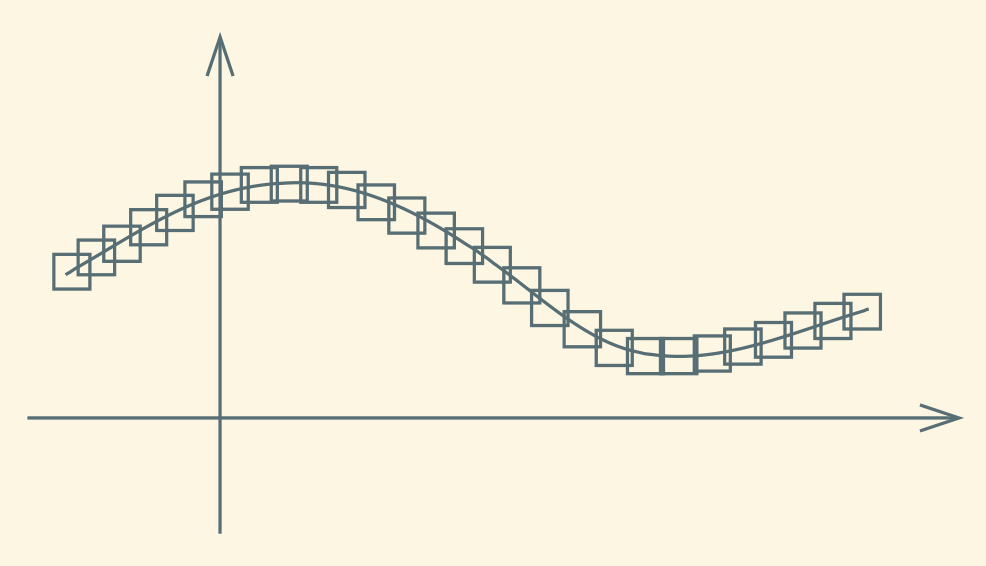
\includegraphics[width=0.7\textwidth]{fig1}
	\end{figure}
\(S \subset \mathbb{R}^n\) possui \textit{\textbf{medida nula}} se \(\forall  \varepsilon >0\) existe \(\{c_i\}_{i=1}^\infty\) cubos (ou bolas) tais que \[S \subset \bigcup_{i=1}^\infty \operatorname{Vol}(c_i)<\varepsilon\]
\end{defn}

\begin{prop}\leavevmode
	\begin{enumerate}
	\item Uma união enumerável de conjuntos de medida nula tem medida nula.
	\item \(f : \mathbb{R}^n \to \mathbb{R}^n\) \(C^1\) e \(S \subset \mathbb{R}^n\) tem medida nula, então \(f(S)\) tem medida nula.
	\end{enumerate}
\end{prop}

\begin{proof}\leavevmode
\begin{enumerate}
\item \(\{S_i\}\) enumerável de medida nula, para cada $i$ você pode escolher cubos \(C^i_1,C^i_2,\ldots\) que cobren \(S_i\) e tal que a soma dos volumes deles é menor do que \(\sum_j \operatorname{Vol}(C^i_j)<\frac{\varepsilon}{2^i}\). Vai ver que a soma dos volumeis variando tanto \(i\) como \(j\) da \(\varepsilon\).

\item (Foto)
\end{enumerate}
\end{proof}

\begin{defn}\leavevmode
	\(X\) variedade diferenciável. \(S \subset X\). Dizemos que \(S\) tem \textit{\textbf{medida nula}} se \(\exists \{U_i\}_{i=1}^\infty\) cobertura aberta de \(S\), i.e. \(\bigcup_{i=1}^\infty S_i \supset S\), e cartas \(\varphi_i:U_i\to \mathbb{R}\) e \(S_i \subset U_i\) e \(\varphi(S)\) tem medida nula.

	O más bien: sólo el chiste es que cada conjunto tiene medida en \(\mathbb{R}^n\) cuando proyectas con cualquier carta.
\end{defn}

\begin{coro}\leavevmode
	\begin{enumerate}
	\item \(\{S_i\}_{i=1}^\infty\).  \(S_i \subset X\) medida nula, entao \(\bigcup_{i \in \mathbb{N}}S_i\) tem medida nula.
	\item \(X^n, Y^n\) variedades, \(f:X \to Y\) suave, \(S \subset X\) medida nula. Então \(f(S)\) tem medida nula.
	\end{enumerate}
\end{coro}

\begin{prop}\leavevmode
\(Y^n\) variedade, \(X^m \subset Y^n\) subvariedade de dimensão \(m <n\). Então \(X\) tem medida nula.
\end{prop}

\begin{proof}\leavevmode
É simplesmente levar para \(\mathbb{R}^n\): considera \(X_i\) como a parte de \(X\) que está den'de cada  \(U_i\) no atlas de \(Y\) e vai ver que ele tem dimensão menor. Daí é só provar que subespaços (acho que lineares) de dimensão menor em \(\mathbb{R}^n\) tem dimensão menor.
\end{proof}

\begin{coro}[Minisard]\leavevmode
\(X^m,Y^n\) variedades \(m<n\)  e \(f:X \to Y\) suave. Então \(f(X)\) tem medida nula.
\end{coro}

\begin{proof}\leavevmode
Aqui se usa o corolário: usar a inclusão \(\iota:X \to X \times \mathbb{R}^{n-m},x \mapsto (x,0)\), compor com \(\tilde{f}:X \times R^{n-m}\to Y\), \((x,y) \mapsto  f(x)\). Então \(\tilde{f}(i(X))=f(X)\). O lance é que \(\iota(X)\) é uma subvariedade de codimensão positiva, então pela prop anterior tem medida nula. Daí $f(X)$ também.
\end{proof}

\begin{coro}[Versão fácil do teorema de mergulho de Whitney]\leavevmode
	Se \(X^n\) variedade diferenciável compacta, então existem 
	\[X \hookrightarrow \mathbb{R}^{2n+1},\qquad  X\rightlooparrow \mathbb{R}^{2n}\]
\end{coro}

\begin{thm}[Difícil de Sard]\leavevmode
\[X \hookrightarrow \mathbb{R}^{2n},\qquad  X\rightlooparrow \mathbb{R}^{2n-1}\]
\end{thm}

\begin{proof}[Prova do corolário]\leavevmode
\begin{enumerate}[label=\textbf{Step \arabic*}]
\item Mergulhar a variedade num espaço euclidiano \textit{grande}. Pegue um atlas finito \(\{(U_i,\varphi_i)_{i=1}^k\}\), note que \(\varphi_i:U_i \to \mathbb{R}^n\) são mergulhos.

\begin{thing6}{Ideia}\leavevmode
\begin{align*}
	\Phi: X &\longrightarrow \mathbb{R}^n\times \mathbb{R}^n \times\ldots\times \mathbb{R}^n \subset \mathbb{R}^{nk} \\
	p &\longmapsto (\varphi_1(p),\varphi_2(p),\ldots
\end{align*}
Isso não da. Para fazer bem precisamos de uma partição da unidade \(\{\rho_i\}_{i=1}^k\) subordinada a \(\{U_i\}_{i=1}^k\) sobertura. Defina \(\rho_i\varphi_i:X \to \mathbb{R}^n\) como sendo zero fora do conjunto bom; note que essa função não é mais um mergulho, mas tudo bem. Agora faça \(X \to (\mathbb{R}^n)^k\times \mathbb{R}^k=\mathbb{R}^{nk+k}\)
\begin{align*}
	\Phi: X &\longrightarrow (\mathbb{R}^n)^k \times\mathbb{R}^k = \mathbb{R}^{nk+k} \\
	p &\longmapsto \Big((\rho_1 \varphi_1)(p),\ldots,\Big(\rho_k \varphi_k)(p)\Big)
\end{align*}
\begin{exercise}[Importante]\leavevmode
	Mostre que \(\Phi\) é uma imersão injetiva.
\end{exercise}
\end{thing6}

\item \textbf{Afirmação:}
	\[X \hookrightarrow  \mathbb{R}^n \implies \begin{cases}
		X \hookrightarrow \mathbb{R}^{N-1}\qquad &\text{ se $N>2n+1$}  \\
		X \rightlooparrow \mathbb{R}^{N-1} \qquad &\text{se $N>2n$.} 
	\end{cases}\]
\begin{proof}[Prova da afirmação]\leavevmode
Vamos projetar a variedade mergulhada em \(\mathbb{R}^n\) no plano ortogonal a algum vetor \(a \in \mathbb{R}^n\). Resulta que
\begin{exercise}\leavevmode
	\begin{align*}
	g: X \times X \times \mathbb{R} &\longrightarrow \mathbb{R}^N \\
	(x,y,t) &\longmapsto \operatorname{pr}_a \circ f
\end{align*}
é injetiva.
\end{exercise}
\end{proof}

\item \textbf{Ideia:} ver que em quase todo ponto podemos projetar.

Considere agora o mapa pusforward que pega um vetor tangente e manda mediante $f$:
\begin{align*}
	h: TX &\longrightarrow \mathbb{R}^N \\
	(x,v) &\longmapsto (Df)_xv
\end{align*}
Agora note que
\begin{thing4}{Afirmação}\leavevmode
\(a \not\in \operatorname{Im}(h) \iff \operatorname{pr}_a \circ f\) é uma imersão \(\iff\) \(D(\operatorname{pr}_a \circ f)_a\) é injetiva para toda $x$.
\end{thing4}

\item A prova termina usando minisard: as imagens de $g$ e de \(h\) tem medida nula. Mesmo a união delas. Então existe um ponto fora dessa união.
\end{enumerate}
\end{proof}

\begin{defn}\leavevmode
Sejam \(X^m, Y^k\) variedades, \(f:X \to Y\) suave, dizemos que
\begin{enumerate}[label=(\alph*)]
	\item \(x \in X\) é \textit{\textbf{ponto crítico}} se o posto de \(Df_x\) é menor do que \(\operatorname{min}(m,n)\). (\(\iff\)não é surjetiva I think) {\color{6}Aula 7: essa definição é que a derivada não é de posto máximo. Isso permete que o domínio tenha pontos regulares, así fez Sard e  \cite{gui2}, mas não \cite{lee}, \cite{gui}.}
\item \(x \in X\) é \textit{\textbf{ponto regular}} se posto \(Df_x=\operatorname{min}(m,n)\).
\item \(y \in Y\) é \textit{\textbf{valor crítico}} se existe um ponto crítico tal que \(f(x) = y\).
\item \(y \in Y\) é \textit{\textbf{valor regular}} se \(\forall x \in f^{-1}(y)\), \(x\) é valor regular.
\end{enumerate}
\end{defn}

\begin{thm}[Sard]\leavevmode
\(f:X \to Y\) suave. Então \(\{\text{valores críticos} \}\) tem medida nula.
\end{thm}

\begin{remark}\leavevmode
\begin{enumerate}
\item Teorema vale se \(f\) é \(C^\ell\), onde \(\ell>\operatorname{max}(m-n,0)\). 

	. \end{enumerate}
\end{remark}

\begin{proof}\leavevmode
\begin{enumerate}[label=\textbf{Step \arabic*}]
\item \textbf{Redução para a versão local.} Supomos que \(X= \mathbb{R}^{m}, Y=\mathbb{R}^n\). \(f:U \subset \mathbb{R}^m \to \mathbb{R}^n\), \(U\) aberto.
	\[\operatorname{Crit}f= \{x \in 0:\text{posto } f'(x) < \operatorname{min}(m,n)\}\]
Então \(f(\operatorname{Crit}(f)\) tem medida nula. Para isso fazemos \textbf{indução em $m$.} \(m=0\) trivial.

\(C_i\) vai ser o conjunto onde as derivadas parciais se anulam até $i$:
 \[C_i=\left\{ p \in U: \frac{\partial^{(\alpha)}}{\partial x^{\alpha}}f_k(p)=0 \forall \alpha, 0<| \alpha|\leq 1, \forall  k \right\}.\]
 Note que \(C_{i+1}\subset C_i \subset C_{i-1}\subset\ldots C_1\subset C:=\operatorname{Crit}f\).

 \begin{thing7}{Objetivo}\leavevmode
 \(f(C)\) tem medida nula.
 \begin{enumerate}[label=\textbf{Paso \arabic*}]
 \item \(f(C_N)\) tem medida nula para algum  \(N \gg 0\). {\color{8}Crucial}
\item \(f(C_i \setminus C_{i+1}\) tem medida nula para toda $i$.
\item \(f(C\setminus C_i\) tem medida nula.
 \end{enumerate}

\begin{enumerate}[label=\textbf{Paso \arabic*}]
\item Podemos supor sem perda de generalidade que \(U\subset\)cubo, a fórmula de Taylor diz que
	\[\|f(x)-f(y)\|_\infty \leq K \cdot \|x-y\|_\infty^{i+1}\]
para todo \(x, y \in C_i\).

Tem que botar \(C_i\) den'de um cubo \(D_j\) que se divide em \(r^m\) cubos de lado \(b/r\). Então  \(f(D_j)\) está contido num cubo em \(\mathbb{R}^n\) de lado \(K \cdot \left(\frac{b}{r}\right)^{i+1}:=R_j \). Também note que pontos den'de \(D_j\) são tq. \(\|x-y\|_\infty \leq  \frac{b}{r}\).

Agora
\[f(C_i) \subset f\left(\bigcup_{j=1}^{r^m}D_j\right) \subset \bigcup_{j=1}^{r^m}f(D_j)\subset \bigcup_{j=1}^{r^m}R_j.\]
Então
\begin{align*}
\sum_{j=1}^{r^m}\operatorname{Vol}(R_j)&=r^m\cdot K^n\cdot \left(\frac{b}{r}\right)^{(i+1)\cdot n}\\
&= \frac{K^n \cdot b^{n(N+1)}}{r^{n(N+1)-m}}
\end{align*}
\end{enumerate}
 \end{thing7}

\item 
\end{enumerate}

\end{proof}

\section{Aula 4}

\subsection{Teorema de Sard}

\begin{thm}[Sard]\leavevmode
\(f: \mathbb{R}^m \to \mathbb{R}^n\) \(C^\ell\), \(\ell >  \operatorname{max}(m-n,0)\). Então \(\{\text{valores críticos} \}\) tem medida nula.
\end{thm}

\begin{proof}\leavevmode
\textbf{Note que} \(\{\text{valores críticos} \}=f(\{\text{ptos críticos} \})\).

Seja \(C=\{\text{ptos críticos de $f$} \}\). Então aproximamos a conjunto onde todas as derivadas parcias são zero com o conjunto \(C_i\) onde as derivadas parciais até \(i\) se anulam. 
\begin{enumerate}[label=\textbf{Passo \arabic*}]
\item \(f(C_N)\) tem medida nula se \(N>\operatorname{max}(m-n,0)\). {\color{6}(Feito na aula pasada.)}
\item \(f(C_i\setminus C_{i+1}\) tem medida nula
\item \(f(C\setminus C_1\) tem medida nula.
\end{enumerate}
Concluimos porque \(f(C)\) é a união de treis conjuntos de medida nula: um por cada passo. Segundo e terceiro passos são com indução em $m$.

Prova:
\begin{enumerate}[label=\textbf{Passo \arabic*}]
\item Feito ontem.
\item A ideia é que podemos dar coordenadas de dimensão 1 menos usando que a derivada \(i+1\) não se anula. (Acho.)
\item É parecido só que um pouco mas dificil. No caso anterior os valores da função \(h\) são zero, aqui não (ver foto). Aqui usamos
	\begin{lemma}\leavevmode
A compact subset whose intersection with every hyperplane has measure zero has measure zero:

\(A \subset\mathbb{R}^n\) compacto tal que \(X \cap \{ x \}\times \mathbb{R}^{n-1}\) tem medida nula em \(\mathbb{R}^{n-1}\) para toda \(x \in \mathbb{R}\). Então \(A\) tem medida nula.
	\end{lemma}
	\begin{proof}[Prova do lema]\leavevmode
	A ideia es pegar uma faixinha de altura $x$ e cobrir esse pedaço de \(A\) com quadradinhos naquele plano \(C^x_j\). Dai, ``como \(A\) é compacto" podemos pegar um \(I_x \subset \mathbb{R}\) intervalo tal que para todo \(y \in I_x\) ($y$ perto de \(x\)), a faixinha de altura $y$ fique contida em \(\bigcup I_x \times C_j^x\)

	{\color{4}\bfseries Ideia.}\hspace{.5em} Como \(A\) é compacto podemos pegar um mini intervalo tal que todas as faixinhas muito pertinho (bom, a parte de \(A\) em cada faixinha) fica den'dos quadrados \(C^x_j\) multiplicados por esse mini-intervalo.

	Agora calculamos os vulmeis. Lembre de análise na reta (ver \cite{lee} lem 6.2, tem que shrink os intervalos) que a soma dos comprimentos dos intervalos \(I_{x_i}\) que conformam uma cobertura esencial (não pode tirar nenhum dos abertos da coberta) de um intervalo \(L\) \textbf{é menor do que duas vezes o tamanho do intervalo}:  \(\sum \operatorname{compr}(I_{x_i})< 2(2L)=4L\).

	Em fim, a soma dos comprimentos é um número finito. Então fica que
	\begin{align*}
	\sum_{i,j}\operatorname{Vol}(I_{x_i} \times C_j^{x_i}&= \sum_i \sum_j \operatorname{Vol}_1(I_x) \operatorname{Vol}_{n-1}(C_j^{x_i})<\varepsilon \sum \operatorname{Vol}_1(I_{x_i}) < 4L\varepsilon.
	\end{align*}
	\end{proof}
\end{enumerate}
\end{proof}

\subsection{Espaço de jatos}

Son como vectores de orden de diferenciabilidad más grande: a ideia é generalizar o espaço tangente e o espaço cotangente \textbf{para derivadas de ordem maior}.

\begin{defn}\leavevmode

	Dos funciones \(f,g:X\to Y\) suaves que mandan \(p\) al mismo punto son equivalentes si existem cartas tales que las derivadas parciales de sus representaciones en coordenadas coinciden hasta orden \(k\).
\end{defn}

Sejam \(X, Y\) variedades diferenciaveis suaves e \(f,g:X \to Y\) suaves. Dizmos que \(f \sim_k g\) em \(p \in X\) se, intuitivamente, as derivadas parciais de \(f \) e \(g\) coincidem até ordem $k$. Isso é inuitivo porque precisamos pegar cartas para isso ficar bem definido: precisamos que existam cartas \((U, \varphi),(V,\psi)\) aoredor de \(p\) e \(f(p)\) tais que
\[\frac{\partial ^{|\alpha|}}{\partial x^\alpha}(\psi \circ f \circ \varphi^{-1}(\varphi(p))=\frac{\partial ^{| \alpha|}}{\partial x^\alpha}(\]
Los \textit{\textbf{jatos}} son gérmenes:
\[J^k(X,Y)_{p,q}=\{f:X \to Y: f(p)=q\}\Big/ \sim_k.\]
Isso generaliza o espaço tangente do seguinte jeito:
\[J^1(\mathbb{R},Y)_{0,q} \cong T_qY.\]
\begin{exercise}\leavevmode
\[J^1(X,\mathbb{R})_{p,0}\cong T_p^*Y.\]
\end{exercise}

\begin{proof}[Solution]\leavevmode
Vamos definir uma correspondência que a cada jato associa um funcional em \(T^*_pM\) pensando que os vetores são classes de equivalência de curvas \([\gamma]\). Pegue um jato \(\sigma\). Esse jato \(\sigma\) tem um representante \(f:X \to \mathbb{R}\) (que manda $p$ a zero). Pegue \(d_pf:T_pX \to \mathbb{R}\), um elemento de \(T_p^* X\). É claro que esta correspondência está bem definida: se \(g : X \to \mathbb{R}\) está relacionada com \( f\), as derivadas parciais delas coincidem em $p$, de forma que \(d_pf=d_pg\). A contenção oposta é evidente: toda forma em \(T_p^*X\) é a diferencial de algum jato já que a base canônica de \(T^*_pX\) está dada por diferenciais de funções em $p$.
\end{proof}
Daí definimos o \textit{\textbf{espaço de $k$-jatos}}:
\[J^k(X,Y):= \bigsqcup_{\substack{p \in X \\ q \in Y}}J^k(X,Y)_{p,q}\]

Então pega um jato \(\sigma \in J^k(X,Y)\). Isso cuspe um \(p\) e um  \(q\) tais que  \(\sigma \in J^k(X,Y)_{p,q}\). Definamos as funções
\[\begin{aligned}
	\alpha: J^k(X,Y) &\longrightarrow X \\
	\sigma &\longmapsto p
\end{aligned}\qquad \qquad \begin{aligned}
	\beta: J^k(X,Y) &\longrightarrow Y \\
	0 &\longmapsto q
\end{aligned}\]

\begin{example}\leavevmode
\(X=U \subset \mathbb{R}^n\), \(Y= V \subset \mathbb{R}^m\) abertos. O que é o espaço de jatos neste caso?

Tem uma bijeção 
\begin{align*}
	: J^k(U,V)_{x,y} &\xrightarrow{\cong}B_{n,m}^k \\
	f &\longmapsto (f_1^k,\ldots,f_m^k)
\end{align*}
Lance: pode pensar que esas funções são polinomias de grau maximo $k$.
\[B^k_{n,m}=\{p: \mathbb{R}^n\to \mathbb{R}^m: p \text{ polinomial de grau \(\leq k\) tal que \(p(0)=0\)} \}.\]

\begin{exercise}\leavevmode
Calcule a dimensão de \(B^k_{n,m}\).
\end{exercise}

\begin{proof}[Solution]\leavevmode
Enquanto eu achei que a dimensão era \(k^m\), porque cada espaço de polinomios (\textit{em uma variável}, sem termo constante) está generado por \(\left<x,x^2,\ldots,x^k\right>\) e temos $m$ deles, errei. Porque são polinomios em $n$ variaveis. Então a base do espaço de polinomios em $n$ variáveis de grau máximo \(k\) e sem termo constante e… o conjunto de monomios linearmente independentes de grau máximo \(k\)

Façamos um polinomio de $n$ variáveis de grau máximo \(k\). Tendo $n$ variáveis, pode pegar só uma delas, ai tem $n$ opções. Pode pegar duas delas, ai tem mais \(n^2\) opções. Tres, quatro, até \(k\) delas. Tem \(\sum_{i=1}^k n^i\) diferentes monomios. {\color{2}Mas…} o que acontece com a ordem?

De acordo com ChatGPT, o problema fica melhor quando pensamos que a cada variável (=indeterminada \(x_i \in k[x_1,\ldots,x_n]\)) de um monómio associamos um número inteiro maior o igual de que 0, o exponente da variável. Daí a quantidade de monomios de grau \(i\) é simplesmente a quantidade de vetores inteiros não negativos \(a_j\) tais que \(\sum a_j=i\). Isso é o mesmo que a quantidade de formas de acomodar \(i\) bolinhas em $n$ caixinhas. Isso é o mesmo que a quantidade de formas de acomodar \(n-1\) divisionsinhas numa lista de \(i\) bolinhas (porque todas as bolinhas são iguais). Então são \(i + n-1\) coisas (divisionsinhas ou bolinhas) numa linha, e nesses \(i + n-1 \) lugares escolhemos \(n-1\) para botar as divisionsinhas. O resultado é \(\binom{i+n-1}{n-1}\). Somar sobre \(i\). Elevar à $m$.
\end{proof}
\[\begin{tikzcd}
J^k(U,V)\arrow[rr,"\cong"]\arrow[dr,"\alpha",swap]&&U \times V \times B^k_{n,m}\arrow[dl,"\operatorname{pr}_1"]\\
&U
\end{tikzcd}\]


Creo que: definimos \(f^k_i\) como as "partes sem constante dos polinómios de Taylor de ordem $k$ das coordenadas de $f$",
{\color{7}CREO QUE la idea es que la clase de equivalencia \([f]\)  está determinada por los principios de los polinomios de Taylor de sus funciones coordenadas.}

No entendí esto pero va:
\begin{align*}
	p: \mathbb{R}^n &\longrightarrow \mathbb{R}^m \qquad \text{polinomial}
\end{align*}
\(x_0 \in U, y_0 \in V\), entre aspas:
\["f(x-x_0) = y_0+p(x-x_0),\]
\(f(U) \subset V.\)
En fim, temos que
\begin{enumerate}
	\item[2.] \(J^1(M,\mathbb{R}) \cong \mathbb{R} \times T^*M\).
	\item[3.] \(J^1(\mathbb{R},M) \cong \mathbb{R} \times TM.\)
\end{enumerate}
\end{example}
Agora o pushforward e o pullback, que basicamente é precompor e poscompor:
\begin{defn}\leavevmode
\begin{enumerate}
\item \(\varphi:Y \to Z\) suave, \(X \) variedade suave. O \textit{\textbf{pushforward}} é
	\begin{align*}
		\varphi_*: J^k(X,Y) &\longrightarrow J^k(X,Z) \\
		[f]_x &\longmapsto [\varphi \circ f]_x
	\end{align*}
\item O  \textit{\textbf{pullback}} é… mas aqui \textbf{precisamos que  \(\psi\) seja difeomorfismo} 
	\begin{align*}
		\psi^*: J^k(X,Y) &\longrightarrow J^k(Z,Y) \\
		[f]_x &\longmapsto [f \circ \psi]_{\psi(x)}
	\end{align*}
\end{enumerate}
\end{defn}

\begin{remark}\leavevmode
\begin{enumerate}
\item \(\sigma \in J^k(X,Y)_{x,y}\), \(\varphi_* \sigma \in J^k(X,Z)_{x,\varphi(y)}\)
\item \(\sigma \in J^k(X,Y)\), \(\psi ^*\sigma \in J^k(Z,Y)_{\psi^{-1}(x),y}\)
\end{enumerate}
\end{remark}

\clearpage
\subsubsection{Estrutura diferenciável no espaço de jatos}

\subsubsection{When dani finally understood this}

Here's how the charts (and the topology) of \(J^k(X,Y)\) is constructed.
\begin{enumerate}
\item Choose charts \((U,\varphi)\) of \(X\) and \((V,\psi)\) of \(Y\).

 \item Take the jet space \(J^{k}(U,V)\) to an euclidean jet space via the induced maps of the charts:
	 \[(\psi^{-1})^*\varphi*:J^{k}(U,V)\to J^{k}(U',V')\]
	where \(U'=\varphi(U)\) and \(V'=\psi(V)\).

\item Now that you are in euclidean space you can compute Taylor polynomials: a  \(k\)-jet \([f]\in J^{k}(U',V')\) has coordinate functions, the Taylor polynomials of which are well-defined up to order \(k\):
	\begin{align*}
		f: U' \subset \mathbb{R}^n &\longrightarrow V' \subset \mathbb{R}^m \\
		x_0 &\longmapsto \Big(f_1(x_0),\ldots,f_m(x_0) \Big)
	\end{align*}
Define
\[T_kf_i(x_0):=\text{Taylor polynomial of \(f_i\) at \(x_0\) up to degree \(k\)}. \]
\item Realise: for every \(k\)-jet \([f] \in J^{k}(U',V')\) its coordinates are:
	\begin{align*}
	\Big(\alpha[f],\beta[f],T_kf_1(\alpha[f]),\ldots,T_kf_m(\alpha[f]) \Big)&\in U' \times V'\times P^k_{n}\times\ldots\times P^k_n\\
	&=U' \times V' \times B^k_{n,m}.
	\end{align*}
	where \(\alpha[f]\) is (the coordinates of) the source, \(\beta[f]\) its target.

{\color{2}\bfseries The point is}\hspace{.5em}that when you take an open set of \(J^k(X,Y)\) you are basically taking an open set of \(X\), an open set of \(Y\), and \textit{an open set in some crazy polynomial space (that is not crazy at all: it's euclidean space!)}. So, its just a product of
\[\text{\textbf{open set in \(X\)} } \times \text{\textbf{open set in \(Y\)} } \times \text{\textbf{crazy euclidean space \(\mathbb{R}^N\)} } \]
Never forget that this is what a basic open set in \(J^k(X,Y)\) looks like.
\end{enumerate}

\subsubsection{how this can also be something else}
\textbf{Now we read the book of Mukherjee}


The space of polynomials of degree \(\leq r\) with constant term equal to zero defined on \(\mathbb{R}^n\) with values in \(\mathbb{R}^m\) is
\[P^r(n,m)=L(\mathbb{R}^n,\mathbb{R}^m)\times L^2_s(\mathbb{R}^n,\mathbb{R}^m) \times \ldots \times L^r_s(\mathbb{R}^n,\mathbb{R}^m)\]
where \(L^k(\mathbb{R}^n,\mathbb{R}^m)\) is the space of \(k\)-multilinear maps \(L(\mathbb{R}^n\times \ldots\times, \mathbb{R}^m\) and the little \(s\) means they are symmetric.

So we also have
\[P^r(n,m)=\underbrace{P^r_n \oplus  \ldots \oplus  P^r_n}_{\text{\(m\) summands} }\]
where \(P^r_n\) is the set of all polynomial functions in \(n\) variables.

\begin{thing2}{Superlemma 8.1.3}[Mukherjee]\leavevmode
Let \(U\subset \mathbb{R}^n_+\) and \(V \subset \mathbb{R}^m\) be open subsets. Then there is a canonical bijection
\begin{align*}
	 h_{U,V}: J^{r}(U,V) &\longrightarrow U \times V \times P^r(n,m)\\
	 j^rf&\longmapsto \Big(p,f(p),Df(p), \ldots, D^r f(p)\Big)
\end{align*}
where \(D^kf\) is the \(k\)th total derivative of \(f\), a \(k\)-multilinear map from \( \mathbb{R}^n\) to \(\mathbb{R}^m\), i.e. an element of \(L^k(\mathbb{R}^n,\mathbb{R}^m)\) defined inductively by taking the derivative of the derivative etc. (Symmetric I think because partial derivatives commute.)


\vspace{4em}
{\color{6}\bfseries Now we see}\hspace{.5em} that two things that are similar and yet very different can be used interchangably: the ``differential coordinates" of a jet (=the part of the coordinates that is not the coordinates in \(X\) nor \(Y\)) can be seen as:
\begin{itemize}
\item the truncated Taylor polynomials of the \(m\) coordinate functions of \(f\) at some  local charts,
\item the total differentials of \(f\) from \(1\) to \(k\).
\end{itemize}

\end{thing2}

\vspace{3em}
{\color{8}\bfseries Last but not least}\hspace{.5em}these open sets are in fact jet spaces of the form \(J^k(U,V)\).

\clearpage
\subsubsection{Lecture notes}

Pegue \(\sigma \in J^k(X,Y)_{p,q}\) e cartas \((U,\varphi)\) de \(p\) e \((V,\psi)\) de $q$. {\color{4}Ideia:} usar o pushforward e o pullback das cartas para levar o problema no \(\mathbb{R}^n\).

\begin{exercise}\leavevmode
Considere
\[J^k(U,V)= \bigsqcup_{\substack{p \in U \\ q \in V}}J^k(X,Y)_{p,q}.\]
Então
\begin{align*}
	J^k(U,V) &\longrightarrow J^k(\varphi(U),\psi(V)) \\
	\sigma &\longmapsto \psi_*(\varphi^{-1})^*\sigma
\end{align*}
é uma bijeção.
\end{exercise}
Então para dar uma estrutura de variedade topológica no espaço de jatos note que também
\[J^k(\varphi(0),\varphi(V))\cong \varphi(0) \times \varphi(V) \times B^k_{n,m}\subset \mathbb{R}^{n+m+ \dim B^k_{n,m}}\]
(lo bueno es que ya sabes cual es la dimension de \(B^k_{n,m}\). Mas não interessa qual é a dimensão: o importante é que o \(B^k_{n,m}\) tem uma base, é um espaço vetorial.)
)
Em fim, tudo isso da uma estrutura de variedade topologica. Para terminhar só temos que ver o que acontece com as mudanças de coordenadas.

\begin{align*}
	\varphi(U) \times \psi(V) \times B^k_{n,m}  &\longrightarrow \tilde{\varphi}(\tilde{U})\times \tilde{\psi}(\tilde{V}) \times B^k_{n,m} \\
	(p,q,f) &\longmapsto \Big(\tilde{\varphi} \circ \varphi^{-1}(p),\tilde{\psi} \circ \psi^{-1}(q) \Big)
\end{align*}
\textbf{Isso é suave!} E isso implica que \(J^k(X,Y)\) é uma \(C^\infty\) variedade de dimensão \(n+m+ \dim B^k_{n,m}\). 


\section{Aula 5: topologia de Whitney}

\begin{enumerate}
\item Terminhamos a estrutura de variedade diferenciavel do espaço de jatos. As cartas são
	\[J^k(\varphi(U),\psi(V)) \xrightarrow{\text{ bijeção} }\varphi(U) \times \psi(U) \times B^k_{n,m}\subset \mathbb{R}^N\]
	lembramos como ver que as funções de transição são suaves {\color{2}(exercício: fazer detalhes)}
\item
	\begin{defn}\leavevmode
	Sejam \(E\), \(B\), \(F\) varoedades dif. \(\pi: E \to B\) suave é um \textit{\textbf{fibrado}} com fibra \(F\) se
	\begin{itemize}
	\item \(\pi\) é uma submersão sobrejetiva.
	\item  para todo \(b \in B\) existe \(U \subset B \) aberto \( U \ni b\) e um difeomorfismo
		\[\begin{tikzcd}
		\pi^{-1}(U)\arrow[rr,"\text{ dif} "]\arrow[dr,"\pi",swap]&&U \times F\arrow[dl,"\operatorname{pr}_1"]\\
		&U
		\end{tikzcd}\]
	\end{itemize}
	\end{defn}

\item  \(\alpha \) e \(\beta\) são fibrados. Também \(\alpha \times \beta: J^k(X,Y)\to X \times Y\). As fibras do último são difeomorfas a um espaço vetorial (polinomios B) mas esse difeomorfismo não induzem estrutura de espaço vetorial. Caso \(Y=\mathbb{R}^n\) pode sim pq os jatos são funções em \(m\mathbb{R}^n\), assim pode botar estrutura de espaço vetorial nas fibras.
\item Para cada função  \(f \in C^\infty(X,Y)\) temos uma \textbf{seção} de \(J^k(X,Y)\) chamada \(j^k f:X \to J^k(X,Y)\) dada por \(x \mapsto  [f]_x\).

\item  Topologia de Whitney \(C^k\) defn.
\item  Lema: \(k \leq  \ell \implies  W_k \subset W_\ell\).
\item Def: a topologia \(C^ \infty\) \textit{\textbf{de Whitney}} é a topologia gerada por \( \bigcup_{k=1}^\infty W_k\) onde \(W_k\) e a \(k\)-ésima. ``\(U\) é aberto em \(C^\infty\)" se para todo \(x\in U\) existe \(V\) aberto em algum \(C^k\) (para todo \(x\) existe \(V\) e existe \(k\)) tais que \(x \in V \subset U\).
\item  Def: Seja \(\delta : X \to \mathbb{R}_+=(0,\infty)\) e \(f \in C^\infty(X,Y)\) definimos a \textit{\textbf{\(\delta\)-bola}} como
	\[D_\delta(f)=\{f \in C^\infty(X,Y)|d(j^kf(x),j^kg(x))<\delta(x)\forall x \in X\}\]
	onde $d$ é qualquer métrica em \(J^k(X,Y)\). {\color{6}(A distancia entre as derivadas é muito pequena.)}
\item Prop: \(\{B_\delta(f): \delta:X \to \mathbb{R}_+\}\) é uma base local centrada em \(f\) da topologia \(C^k\), i.e.
	\begin{itemize}
	\item \(B_\delta(f)\) é aberto.
	\item \(\forall  \mathcal{W} \ni f\) aberto, existe \(\delta\) tal que \(B_\delta(f) \subset \mathcal{W}\).
	\end{itemize}
\item Fix: a locally finite atlas \(\Phi\) of \(X\) with a \(\Subset\) cover (every open set of the cover contains an open subset whose closure is compact and contained in the original open set), an atlas \(\Psi\) of \(Y\), e uns números positivos \(\mathcal{E}=\{ \varepsilon_i\}\), e uma função \(f \in C^\infty(X,Y)\). Então a topologia gereada por (foto) coincide com a topologia \(C^k\).
\item Obs: quando \(X\) é compacto, \(\delta_n=\frac{1}{n}\), \(\{B_{\delta_n}(f)\}\) é uma base local da topologia \(C^k\).
\item Prop: seja \(\{ f_n\}_{n \in \mathbb{N}} \subset C^\infty(X,Y)\), \(f_n \xrightarrow{C^k}f\). Então existe \(K \subset X\) compacto tal que \(f_n \equiv f\) em \(X \setminus K\) e \(j^k f_n \xrightarrow{u}j^kf\) em \(K\).
\end{enumerate}


\section{Aula 6: topologia de Whitney (cont.). Teoremas de transversalidade.}

\subsection{Topologica de Whitney (cont.)}

\begin{enumerate}
\item Lembrança das topologias \(C^k\) e \(C^\infty\).
\item \(X\) variedade não compacta existe \(\{ K_n\}\) compactos tais que \(K_n \subset \int (K_{n+1}\) e \(\bigcup_{n \in N} K_n=X\). Também existe \(\rho: X \to \mathbb{R}_+\),  \(\rho|_{K_{2n+1}\setminus K_{2n}}=2\). \(\rho\) é própria.
\item  Em toda variedade existe uma métrica completa (análise em variedades…).
\item Definição de espaço de Baire.
\item Teo (Prop 3.3). Se \(X, Y\) são variedades suaves, então \(C^\infty(X,Y)\) é um espaço de Baire na topologia \(k=1,2,\ldots,+\infty\).
\item Prop 3.\(X, Y\) variedades diferenciaveis \( j^k : C^\infty(X,Y)\to C^\infty(X, J^k(X,Y))\) é contínua em \(C^\infty\).
\item  \(\phi: Y \to Z \) suave então \(\phi_*: C^\infty(X,Y)\to C^\infty(X,Z)\), \(f \mapsto \phi \circ f\) é contínua em \(C^\infty\). Também \(C^\infty(X,Y) \times C^\infty(X,Z)\to C^\infty(X, Y \times Z)\), \(f, g) \mapsto f \times g\).
\end{enumerate}

\subsection{Teoremas de transversalidade}

A ideia é que a transervsalidade é uma condição generica.

\begin{enumerate}
\item Def: \(X,Y\),  \(f \in C^\infty(X,Y)\), \(W \subset Y\) subvariedade. \(f\) é \textit{\textbf{transversal}} a \(W\) se para todo  \(x \in f^{-1}(W)\),
	\[df_x(T_xW)+T_{f(x)}W=T_{f(x)}Y.\]
\item Obs. Isso impoe restrições sobre as dimensoes: se \(f \pitchfork W\) e \(f^{-1}(W)\neq \varnothing.\) Então \(\dim X + \dim W \geq \dim Y\).

	\begin{remark}[\cite{gui}, p. 35]\leavevmode
	Why can't two curves in \(\mathbb{R}^3\) never intersect transversally (except if they do not intersect at all)? Doesn't make sense because of course they can intersect transversally, right? what happens is that \textit{by a small deformation of either curve, one can abruptly pull the two enteirly apart; their intersection is not stable}:
	\begin{figure}[H]
		\centering
		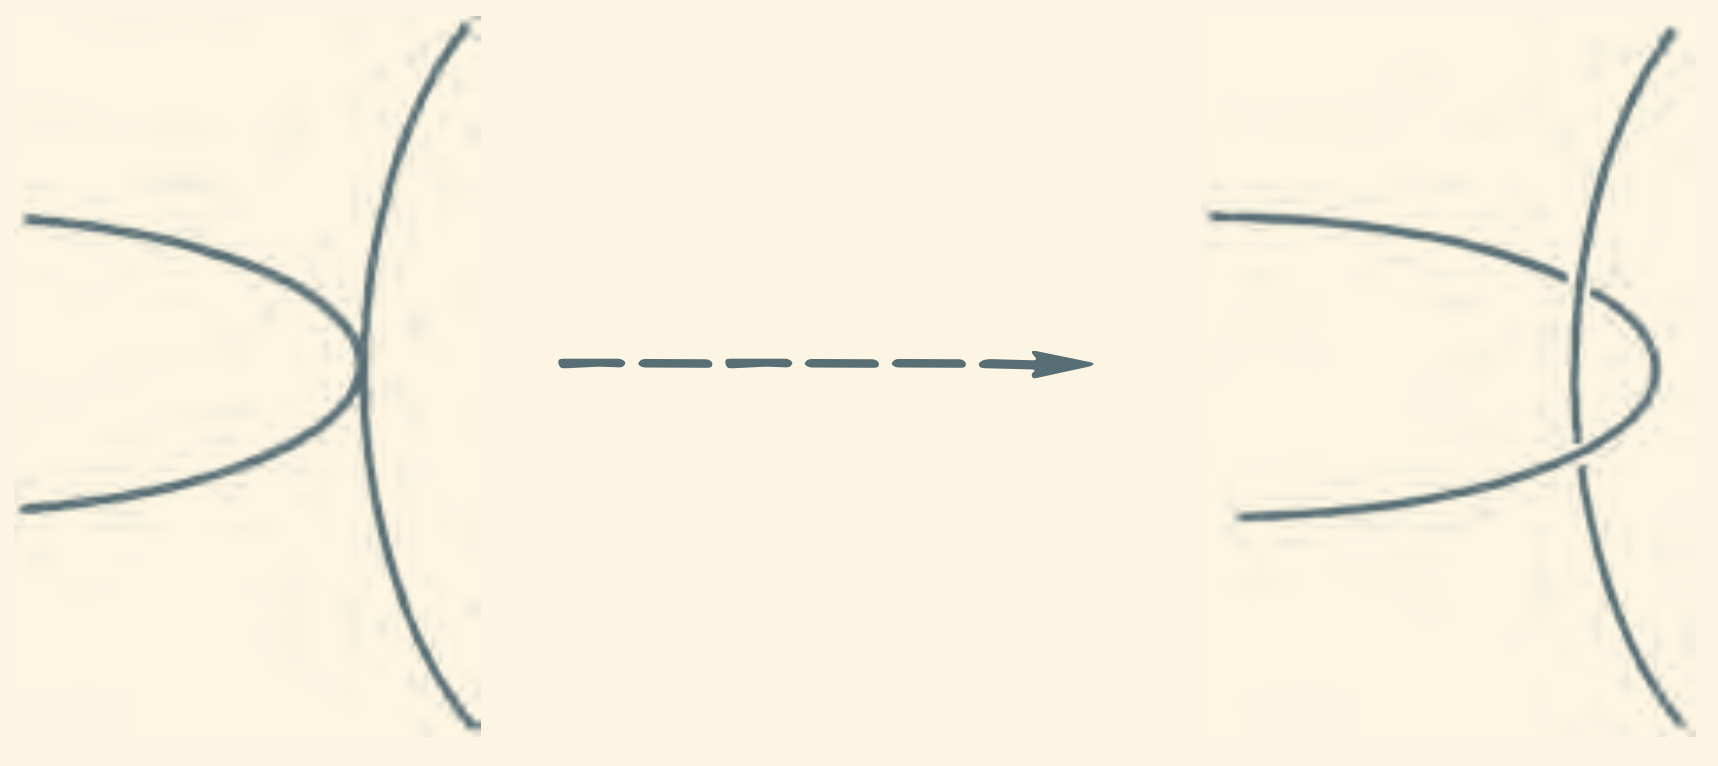
\includegraphics[width=0.7\textwidth]{fig2}
		\caption*{}
	\end{figure}
	\end{remark}
\item Teorema muito importante. \(X,Y\) variedades suaves \(f \in C^\infty(X,Y)\), \(W \subset Y\) subvariedade, \(f \pitchfork W\) e \(f^{-1}(W) \neq  \varnothing\). Então \(f^{-1}(W)\subset X\) é uma subvariedade e \(\operatorname{codim}f^{-1}(W)=\operatorname{codim}(W)\).

	Outra encarnação do teroema da função inversa.

	\begin{remark}[\cite{gui}, p. 29]\leavevmode
	When \(W\) is just a single point, its tangent space is the zero subspace of \(T_y(Y)\). Thus \(f\) is transversal to \(y\) if \(df_x[T_x(X)]=T_y(Y)\) for all \(x \in f^{-1}(y)\) \textbf{which is to say that \(y\) is a regular value of \(f\)}. So transversality includes the notion of regularity as a special case. 
\end{remark}
\end{enumerate}

\section{Aula 7}



\begin{enumerate}
\item Prop: Sejam \(X,Y\) variedades e \(W \subset Y\) subvariedade fechada como subconjunto. \[T_W:= \{f \in C^\infty(X,Y): f \pitchfork W\}\]
é aberto em \(C^\infty\).

{\color{7}A ideia é que podemos perturbar variedades que se intersectam transversalmente, e isso fica transversal que podemos perturbar variedades que se intersectam transversalmente, e isso fica transversal.}

\item Prop: Sejam \(X,Y,B\) variedades, \(W \subset Y\) subvariedade, \(j:B \to C^\infty(X,Y)\) (não podemos supor que \(j\) é contínua. Considere também
\begin{align*}
	\Phi: X \times B &\longrightarrow Y \\
	(x,b) &\longmapsto j(b)(x).
\end{align*}
Suponha que \(\Phi \pitchfork W\).

Então \(\{ B \in B : j(b) \pitchfork W\}\) é denso em \(B\). (Também é verdade que esse conjunto tem medida total.)
	
\item Corolário 4.7.
\item Teorema de transversalidade de Thom. (Formulação.)
\item Coro 4.11. (Formulação.)

\end{enumerate}

\section{Aula 8: teorema de transversalidade de Thom; multijatos}

\subsection{Teorema de transversalidade de Thom}

\begin{thm}[de transversalidade de Thom]\leavevmode
Sejam \(X, Y\) variedades diferenciáveis, \(W \subset J^k(X,Y)\) subvariedade. Então
\[\{ d \in C^\infty (X,Y): j^kf \pitchfork W\}\]
é residual (=interseção de abertos densos).

(Se \(W\) é fechado, então o conjunto também é aberto.)
\end{thm}

\begin{proof}\leavevmode
Primeiro, para o último comentário ali entre paréntese, note que se \(W\) é fechado,
\[U=\{g \in C^\infty (X,J^k(X,Y)):g \pitchfork W\}\]
é aberto. Note que \(T_W= (j^k)^{-1}(U)\).

Como \(j^k: C^\infty (X,Y) \to C^\infty (X,J^k(X,Y))\) é contínua, \(T_W\) é aberto.

\textbf{Começa a prova.} $\mathsf{OK}$ então pegue \(\sigma \in W\). Seja \(W_\sigma \subset W\)  uma vizinhança, e cartaso \(\varphi_\sigma: U_\sigma \to \mathbb{R}^n\), \(\psi_\sigma:V_\sigma \to \mathbb{R}^m\) tais que
\begin{enumerate}
\item \(\alpha(\sigma) \in U_\sigma\) \(\beta(\sigma) \in V_\sigma\).
\item \(\overline{W}_\sigma\), \(\overline{U}_\sigma\) compactos.
\item \(\alpha(\overline{W}_\sigma) \subset U_\alpha\), \(\beta(\overline{W}_\sigma) \subset V_\sigma\).
\item \(\psi_\sigma(V_\sigma) = \mathbb{R}^m\).
\end{enumerate}
Então beleza. Agora pegue
\[T_\sigma=\{f \in C^\infty (X,Y): j^kf \pitchfork W \text{ em } \overline{W}_\sigma\}\]
Então
\[\bigcap_{\sigma \in W}T_\sigma=T_W.\]
Como \(W\) é 2-enumerável, podemos escolher \(\{\sigma_n\}_{n \in \mathbb{N}}\) tal que \(\bigcup_{n \in \mathbb{N}}W_{\sigma_n}=W\). Logo
\[ \bigcap_{n \in \mathbb{N}}=T_W.\]
\begin{claim}\leavevmode
\(T_\sigma\) é aberto e denso.
\end{claim}

\begin{proof}[Prova da afirmação]\leavevmode
\begin{prop}[da aula passada modificada]\leavevmode
\(X,Y\) variedades dif. \(W\subset Y\) subvariedade, \(W' \subset W\) fechado em \(Y\). Então
 \[\{f \in C^\infty (X,Y): j^kf \pitchfork W \text{ em } W'\}\]
é aberto.
\end{prop}
Ussando essa proposição é o fato de que \(j^k\) é contínua, mostramos que \(T_\sigma\) é aberto.

{\color{6}
Para ver que \(T_\sigma\) é denso considere \(f \in C^\infty (X,Y)\). Vamos construir \(\{ g_n\}\subset C^\infty (X,Y)\) tal que \(g_n \xrightarrow{C^\infty }f\) e \(g_n \in T_\sigma\).}

Vamos escolher
\[\rho_1:\mathbb{R}^n\to[0,1]\qquad \qquad \rho_2:\mathbb{R}^m\to [0,1]\]
suaves, \(\rho_1 \equiv 1\) numa vizinhança de \(\varphi_\sigma(\alpha(\overline{W}_\sigma))\), \(\rho_2 \equiv 1\) numa viz. de \(\psi_\sigma(\beta(\overline{W}_\sigma))\), \(\operatorname{supp}\rho_1, \operatorname{supp}\rho_2\) compactos (partição da unidade).

Seja \(B=\{\text{funções polinomiais de \(\mathbb{R}^n \to \mathbb{R}^n\) de grau \(\leq k\)} \} \cong \mathbb{R}^m \oplus  B^k_{n,m}\).

Para \(b \in B\), definimos \( g_b: X \to Y\), 


\[g_b=\begin{cases}
	\psi^{-1}_\sigma(\psi_\sigma(f(x))+\rho_2(\psi_\sigma(f(x))\rho_1(\varphi_\sigma(x))\cdot b(\varphi_\sigma(x))),\qquad &\text{se }x \in U_\sigma\text{ e } f(x) \in V_\sigma  \\
	f(x)\qquad &\text{ se } x \not \in U_\sigma \text{ e } f(x) \not \in V_\sigma
\end{cases}\]
\(g_0=f\).

\paragraph{Intuition for \(g_b\) by ChatGPT.} 
The function \(g_b\) is a smooth perturbation of \(f\) designed to ensure \(j^k g_b \pitchfork W\) in \(\overline{W}_\sigma\). Locally, near \(\overline{W}_\sigma\), \(g_b\) behaves like \(f\) plus a polynomial perturbation \(b(\varphi_\sigma(x))\), where \(b \in B\) spans the \(k\)-jet space. The partition of unity functions \(\rho_1, \rho_2\) localize the perturbation to a compact region, ensuring \(g_b\) is globally smooth and matches \(f\) outside this neighborhood.

Agora:
\begin{align*}
	\Phi: X \times B &\longrightarrow J^k(X,Y) \\
	(x,b) &\longmapsto j^kg_b(x)
\end{align*}

\paragraph{Dependence of \(g_b\) on \(b\).} 
For each \(b \in B\), where \(B\) is the space of polynomials of degree \(\leq k\) in the local coordinates \(\varphi_\sigma(x)\), there is a corresponding perturbation \(g_b\). The choice of \(b\) determines how \(g_b\) modifies \(f\) locally near \(\overline{W}_\sigma\). The perturbation:
\begin{itemize}
    \item Is localized to \(\overline{W}_\sigma\) by the partition of unity functions \(\rho_1\) and \(\rho_2\), ensuring \(g_b = f\) outside \(U_\sigma\).
    \item Explores all possible modifications in the \(k\)-jet space \(B^k_{n,m}\), making the construction rich enough to enforce transversality.
\end{itemize}
While \(b\) can be chosen freely from \(B\), the perturbation is controlled, smooth, and compactly supported, ensuring \(g_b\) remains globally well-behaved.


\textbf{Ideia:} \(\Phi \not{\pitchfork} W\).

Seja \(\varepsilon=\frac{1}{2}\operatorname{dist}(\psi_\sigma(\beta(\overline{W}_\sigma)),\rho^{-1}_2([0,1)))>0\).

\[\tilde{B}=\{b \in B: \|b(x)\|<\varepsilon \forall  x \in \operatorname{sup p} \rho_1\}\]
aberto, \(0 \in \tilde{B}.\)


\paragraph{The subset \(\tilde{B}\) (GPT).} 
The set \(\tilde{B}\) is a subset of the polynomial space \(B\), defined as:
\[
\tilde{B} = \{b \in B : \|b(x)\| < \varepsilon \, \forall x \in \operatorname{supp} \rho_1\},
\]
where \(\varepsilon = \frac{1}{2} \operatorname{dist}(\psi_\sigma(\beta(\overline{W}_\sigma)), \rho_2^{-1}([0,1))) > 0\). This means that \(\tilde{B}\) contains only those polynomials \(b(x)\) whose values are bounded by \(\varepsilon\) within the support of \(\rho_1\). The set \(\tilde{B}\) is open in \(B\), and \(0 \in \tilde{B}\).

\(\tilde{\Phi}:\Phi\Big|_{X \times \tilde{B}}X \times \tilde{B} \to J^k(X,TY)\) é um difeomorfismo local numa viz. de \((x,0)\), onde  \(\Phi(x,b) \in \overline{W}_\sigma.\)

\((x,b)\) t.q. \(\Phi(x,b) \in \overline{ W}_\sigma\). \(j^k g_b(x) \implies x \in \alpha (\overline{W}_\sigma)\), \(g_b(x)=\beta (\Phi(x,b))\).

\[\Psi_b(g_b(x))=\Psi_\sigma(f(x))+\rho_2(\psi_\sigma(f(x))\rho_1(\varphi_\sigma(x))b(\varphi_\sigma(x)).\]
\[\|\Psi_\sigma(g_b(x))-\psi_\sigma(f(x))\| \leq  \|b(\varphi(x))\|<\varepsilon.\]
Então
\[\rho_2(b(\varphi_\sigma(x)))=1.\]

\[g_b(x)=\psi^{-1}_\sigma(\psi_\sigma(f(x))+b(\varphi_\sigma(x)))\]
\[g_b'(x)=\psi^{-1}_\sigma(\psi_\sigma(f(x))+b'(\varphi_\sigma(x))\]
para \(b'\) suficientement próxima de  $b$. \textbf{Isso implica que \(\Phi\)} é um difeomorfismo local para todo \((x,b) \in \Phi^{-1}(\overline{W}_\sigma\).

\paragraph{Summary of \(\tilde{B}\) and its Role (GPT).}
The set \(\tilde{B} = \{b \in B : \|b(x)\| < \varepsilon \, \forall x \in \operatorname{supp} \rho_1\}\), where 
\(\varepsilon = \frac{1}{2} \operatorname{dist}(\psi_\sigma(\beta(\overline{W}_\sigma)), \rho_2^{-1}([0,1))) > 0\), defines a controlled subset of perturbations. Perturbations \(b \in \tilde{B}\) ensure that:
\begin{itemize}
    \item The map \(\tilde{\Phi} = \Phi\big|_{X \times \tilde{B}} : X \times \tilde{B} \to J^k(X, Y)\) is a local diffeomorphism near \((x, 0)\), allowing smooth control of \(j^k g_b\).
    \item For \((x, b)\) such that \(\Phi(x, b) \in \overline{W}_\sigma\), we have \(x \in \alpha(\overline{W}_\sigma)\) and \(g_b(x) = \beta(\Phi(x, b))\), ensuring the perturbation is relevant to \(\overline{W}_\sigma\).
    \item The bound \(\|\Psi_\sigma(g_b(x)) - \psi_\sigma(f(x))\| < \varepsilon\) ensures the perturbation remains localized, with \(\rho_2 = 1\) in the active region, maintaining smoothness and compact support.
\end{itemize}
This construction ensures \(g_b\) perturbs \(f\) only where needed, while staying smooth and controlled globally.

Logo \(\tilde{\Phi}\) é submersão para todo \(x \in \tilde{\Phi}^{-1}(\overline{W}_\sigma)\).

Logo \(d \tilde{\Phi}_{(x,b)}(T_{(a,b)}(X \times \Big)+ T_{\tilde{\Phi}(x,b)}W=T_{\tilde{\Phi}(x,b)}(J^k(X,Y)) \implies \tilde{\Phi} \pitchfork W\) em \(X \times \tilde{B}\).

Pelo lema da aula passada
\[j^kg_b=\Phi_b \pitchfork W\]
para um conjunto denso de \(b \in \tilde{ B}\). Então existe \(b_n \to 0\) tal que \(j^k g_{b_n} \pitchfork W\) em \(\overline{W}_\sigma\), \(g_{b_n}\xrightarrow{C^\infty }f\). (Tem uma conta aqui para ser feita.)

\paragraph{Final Step of the Proof.}
The map \(\tilde{\Phi}: X \times \tilde{B} \to J^k(X, Y)\) is a submersion on \(\tilde{\Phi}^{-1}(\overline{W}_\sigma)\), meaning:
\[
d\tilde{\Phi}_{(x,b)}(T_{(x,b)}(X \times \tilde{B})) + T_{\tilde{\Phi}(x,b)}W = T_{\tilde{\Phi}(x,b)}(J^k(X,Y)).
\]
This implies \(\tilde{\Phi} \pitchfork W\) on \(X \times \tilde{B}\).

By a previous lemma, for a dense subset of \(b \in \tilde{B}\), we have:
\[
j^k g_b = \tilde{\Phi}_b \pitchfork W \text{ on } \overline{W}_\sigma.
\]
Thus, there exists a sequence \(b_n \to 0\) in \(\tilde{B}\) such that:
\[
j^k g_{b_n} \pitchfork W \text{ on } \overline{W}_\sigma, \quad \text{and} \quad g_{b_n} \xrightarrow{C^\infty} f.
\]
This concludes the proof by showing that \(f\) can be approximated arbitrarily closely by maps achieving transversality.


\end{proof}

\end{proof}

\begin{coro}[da demostração]\leavevmode
Sejam \(X, Y\) variedades, \(W \subset J^k(X,Y)\) subvariedade, agora já sei que \(\alpha(\overline{W}) \subset U\), \(U\) aberto de \(X\). {\color{6}``So preciso modificar a função num conjunto aberto, não preciso modificar a função globalmente."}

Então existe \(g \in \mathcal{V}\) tal que \(j^kg \pitchfork W\) \textbf{e \(g \equiv f\) em \(X\setminus U\)}.
\end{coro}

\begin{coro}[Versão simples da transversalidade]\leavevmode
\begin{enumerate}[label=(\alph*)]
\item \(X,Y\) variedades, \(W \subset Y\) subvariedade. Então
\[\{ f \in C^\infty (X,Y): f \pitchfork W\}\]
é denso.

Se \(W\) é fechado, então esse conjunto é aberto.
\item \(U_1,U_2\subset X\)abertos, \(\overline{U_1}\subset U_2\). Então existe \(g \in C^\infty (X,Y)\) tal que \(f \equiv g\) em \(U_1\), \(g \pitchfork W\) em \(X \setminus U_2\). (É só aplicar o corolário para caso de 0-jatos.
\end{enumerate}
\end{coro}

\subsection{Multijatos}
Um pouco mais de teoria para obter corolários bonitos.

\(X,Y\) variedades, \(s \in \mathbb{N}\).
\[X^{(s)}=\{(x_1,x_s)\in X^s: x_1 \neq  x_j, i\neq j\}\]
(são os pontos que não tem duas coordenadas iguais). Isso é claramente aberto em \(X^s\).

\begin{align*}
	\alpha^s: J^k(X,Y)^s &\longrightarrow X^s \\
	(\sigma_1,\ldots,\sigma_s) &\longmapsto (\alpha(\sigma_1),\ldots,\alpha(\sigma_s))
\end{align*}
O espaço de \textit{\textbf{multijatos}} é o espaço de $s$-jatos tal que cada jato está num ponto diferente:
\[J^k_s(X,Y):=(\alpha^s)^{-1}(X^{(s)})\]
i.e. \((\sigma_1,\ldots,\sigma_s) \in J^k_s(X,Y)\) sse \(\sigma_1=j^kf_i(x_i)\), \(x_i \neq  x_j, \qquad  i \neq  j\).

Note que
\[J^k_s(X,Y) \subset J^k(X,Y)^s\]
é aberto.

E agora
\[\alpha^s: J^k_s(X,Y) \to X^{(s)}\]
fibrado.

Para \(f \in C^\infty (X,Y)\),
\begin{align*}
	j^k_sf: X^{(s)} &\longrightarrow J^k_s(X,Y) \\
	(x_1,\ldots,x_s) &\longmapsto (j^kf(x_1),\ldots,j^kf(x_s))
\end{align*}

\begin{thm}[transversalidade para multijatos]\leavevmode
Sejam \(X,Y\) variedades e \(W \subset J^k_s(X,Y)\) subvariedade.
\[T_w=\{ f \in C^\infty (X,Y):j^k_sf \pitchfork W\}\]
é residual. Além disso, se \(W\) é \textbf{compacto}, então \(T_W\) é aberto.
\end{thm}

\subsection{Imersão e mergulho de Whitney}

Sejam \(X, Y\) variedades, \(\sigma = j^1f(x) \in J^1(X,Y)\), \(\operatorname{rk}\sigma=\operatorname{rk}(df_x:T_xX \to T_{f(x)}Y)\). Definimos o \textit{\textbf{coposto}} como sendo
\[\operatorname{corank}=\operatorname{min}(n,m)-\operatorname{rk}\sigma\]
\begin{lemma}\leavevmode
Seja \(S_r=\{\sigma \in J^1(X,Y): \operatorname{corank}\sigma=r\}\). $f$ é imersão (\(n\leq n\)) ou submersão ( \(n \geq m\)) see \(j^1f(X) \cap \bigcup_{r \geq  1}S_r= \varnothing\).
\end{lemma}

\begin{thm}[Imersão de Whitney]\leavevmode
Sejam \(X,Y\) variedades tais que \(m \geq  2n\). Então
\[\operatorname{Im}(X,Y)= \{ f: X \to Y: f \text{é imersão} \}\]
é aberto e denso.
\end{thm}

\begin{prop}\leavevmode
\(S_r\) é uma subvariedade de codimensão \((n-q+r)(m-q+r)\), onde \(q=\operatorname{min}(m,n)\) (o posto máximo).
\end{prop}

\begin{proof}\leavevmode
\(S_r\) é um fibrado sobre \(X \times Y\) cuja fibra é
\[\{A \in \mathcal{L}(\mathbb{R}^n,\mathbb{R}^m): \operatorname{corank}k=r\}\]
Pega uma transformação linear de posto $r$, \(M \in \mathcal{L}^r( \mathbb{R}^n , \mathbb{R}^m)\), \(q = \operatorname{min} (n,m)\), \(k = \operatorname{rk} M= q-r\). Então
\[[M]=\begin{bmatrix} A& B\\C & D \end{bmatrix} \]
Seja \(U\) uma viz. de \(M\) em \(\mathcal{L} (\mathbb{R}^m,\mathbb{R}^m)\). Pegue \(M' \in U\). Então

\(\begin{bmatrix} M' \end{bmatrix} = \begin{bmatrix} A' & B'\\ C' & D' \end{bmatrix}_{n \times m}\) 

Vamos multiplicar \(M'\) por uma matriz que preserva o rank:
\[\operatorname{rk}M'=\operatorname{rk} \begin{bmatrix} I_k& 0\\-C'(A')^{-1} &  I_{m-k} \end{bmatrix}_{m \times m}M'\]
\[=\operatorname{rk} \begin{bmatrix} A' & B'\\0 & D'-C'(A')^{-1} B' \end{bmatrix} \]
{\color{7}Como é que o posto dessa matriz é \(k\)?} Isso acontece see  \(D'-C'(A')^{-1}B'=0\).

Ou seja, \(M' \in \mathcal{L}^r(\mathbb{R}^n,\mathbb{R}^m) \iff D'-C'(A')^{-1}B'=0\).

\begin{align*}
	\varphi: U \subset \mathcal{L}(\mathbb{R}^n,\mathbb{R}^m) &\longrightarrow \mathcal{L}(\mathbb{R}^{n-k},\mathbb{R}^{m-k}) \\
	[M']=\begin{bmatrix} A' & B'\\ C' & D' \end{bmatrix}  &\longmapsto [D' - C'(A')^{-1}B']
\end{align*}

\[\mathcal{L}^r(\mathbb{R}^n,\mathbb{R}^m) \cap U = \varphi^{-1}(0).\]
Submersão, pois
\[\varphi \begin{bmatrix} A' & B' \\ C' & * \end{bmatrix} =\operatorname{Id}- C' (A')^{-1}B'\]
\[\operatorname{codim} \mathcal{L}^r(\mathbb{R}^n,\mathbb{R}^m)=(n-k)(m-k)=(m-q+r)(n-q+r)\]
\end{proof}

\begin{proof}[Do teorema de imersão de Whitney]\leavevmode
\begin{align*}
\operatorname{Im}(X,Y)&=\{f : j^1f(X) \subset S^0\}\\
&=\{ f : j^1f(X) \cap \bigcup_{r \geq  1}S_r = \varnothing\}.
\end{align*}
\end{proof}

\section{Aula 9}

\subsection{Teorema das imersões injetivas}

\begin{thm}[das imersões injetivas]\leavevmode
\(X^n, Y^m\) variedades dif. \(m \geq  2n+1\),
\[\{f \in C^\infty(X,Y): f \text{ imersão injetiva} \}\]
é residual.
\end{thm}
\begin{proof}\leavevmode
Note que $f$ não é injetiva pode ser dito na linguagem de multijatos assim: \(\exists  (x_1,x_2) \in X^{(2)}\) tal que \(j^0_2f(x_1,x_2) \in X^{(2)}\times \Delta_Y\).

Logramos argumentar que $f$ é injetiva see \(j^0_2f(X^{(2)}) \pitchfork W= \varnothing\) para \(W=X^{(2)}\times \Delta_Y \subset J^0_2(X,Y)\), note que \(\operatorname{codim} W=\dim Y=m\). Dai \(\dim X^{(2)}=2n<m=\operatorname{codim} W\). Dai \(j^0_2 f \pitchfork W \iff j^0_2f(X^{(2)}) \pitchfork W= \varnothing\).

aplicamos teorema de transversalidade de multijatos, obtendo que \(\operatorname{In j}(X,Y)\) é residual, e o resultado segue.
\end{proof}

\begin{lemma}\leavevmode
Seja \(X\) variedade.
\[\operatorname{Pr op}(X, \mathbb{R}^m)=\{f: X \to \mathbb{R}^m: f \text{ é própria} \}\]
é não-vazio e aberto.
\end{lemma}

\begin{proof}\leavevmode
\begin{itemize}
\item \textbf{(Não vazio.)} Pegue \(\rho:X \to \mathbb{R}\) própria. Dai \(i:\mathbb{R} \to \mathbb{R}^m\), \(x \mapsto (x,0,\ldots,0)\) é injetiva e linear, asi \(i \circ \rho\) é própria.

\item \textbf{(Aberto.)} Pegue \(f \in \operatorname{Pr o p}(X,\mathbb{R}^m)\). Pegue \(V \subset J^0(X,\mathbb{R}^m) \cong X \times \mathbb{R}^m\) aberto. Queremos ver que \(f \in M(V) \subset \operatorname{ Pr o p}(X,\mathbb{R}^m)\).

	Defina \(Vx=\{y \in \mathbb{R}^m: d(y,f(x))<1\}.\) O truque e esse!

	\[g \in M(V) \iff d (g(x),f(x))<1 \forall  x \in X \iff j^0 g(X) \subset V\]
	então para \(g \in M(V)\) com \(d(g(x),g(x))<1\)  \(\forall  x \in X\), e asi
	\[g^{-1}(\overline{B_r(0)}\subset f^{-1}(\overline{B_r(0))}\]
	e isso implica que \(g\) é própria.
\end{itemize}
\end{proof}

\subsection{Teorema do mergulho de Whitney}

\begin{coro}[Teorema do mergulho de Whitney]\leavevmode
\(X^m\) variedade, \(X \hookrightarrow  \mathbb{R}^{2n+1}\).
\end{coro}

\begin{proof}\leavevmode
\(\operatorname{Im}(X,Y) \cap \operatorname{Inj}(X,Y)\) é residual, logo denso. Então \(\operatorname{Im}(X,Y) \cap \operatorname{Inj}(X,Y) \cap \operatorname{Pr o p}(X,Y) \neq  \varnothing\), which implies that \(X \hookrightarrow  Y=\mathbb{R}^{2n+1}\).
\end{proof}

\subsubsection{Funções de Morse}

\begin{defn}\leavevmode
\( f \in C^\infty(X)=C^\infty(X,\mathbb{R})\). Um ponto crítico de $f$ é quando a derivada não tem posto máximo, neste caso isso implica que a derivada tem posto 0, ou seja, \(d_pf=0\).
 \[D^2_pf:T_pM \times T_pM \to \mathbb{R}\]
 é uma forma bilinear simétrica. Para mostrar que isso está bem definido quando mudamos de coordanadas necesitamos usar que \(d_pf=0\). Também pode ver isso usando  ``conexões": quando a derivada é zero, temos uma eleção canônica de horizontal bundle e podemos identificar \(T_{(p,\underbrace{v}_{=0})}(TM) \cong T_pM \times T_pM\)
\end{defn}

\begin{defn}\leavevmode
\(p \in \operatorname{Crit}(f)\) é não degenerado se \(D^2f_p\) é não degenerada, i.r. para todo \(v \in T_pM \setminus\{0\}\) existe \(w\) tal que \(D^2f_p(v,w)\neq 0 \iff \left(\frac{\partial^2(f \circ \varphi^{-1}}{\partial x^i \partial x^j}\right) \) é residual.
\end{defn}

\[S^1:= \{ j^1 g(x) \in J^1(X,\mathbb{R}):dg_x=0 \iff \operatorname{corank}\sigma=1\}\]

\begin{prop}\leavevmode
\(p \in \operatorname{Crit}(f)\) é não degenerada \(\iff\) \(j^1f \pitchfork S^1\) em $p$. \(p \in (j^1f)^{-1}(S^1)\)
\end{prop}

\begin{proof}\leavevmode
Se usa que a dimensão de \(X\) é a mesma do que a dimensão de \(\mathcal{L}(\mathbb{R}^{2n},\mathbb{R})\).
\end{proof}

\begin{defn}\leavevmode
\(f \in C^\infty(X)\) é uma \textit{\textbf{função de Morse}} se todo ponto crítico de $f$ é não  degenerado.
\end{defn}

\begin{coro}[da proposição]\leavevmode
$f$ é de Morse \(\iff\) \(j^1 f \pitchfork S^1\).
\end{coro}

\begin{thm}\leavevmode
\(\{f \in C^\infty(X): f \text{ é de Morse} \}\) é aberto denso de \(C^\infty(X,\mathbb{R})\).
\end{thm}

\begin{proof}\leavevmode
\(S^1\) é fechado porque é subvariedade, logo o conjunto das funções de Morse é igual a \(\{f : j^1 f \pitchfork S^1\}\) é aberto e denso pelo teorema de Thom.
\end{proof}

\subsection{Teoria de interseção}

\subsubsection{Preliminares: variedades com bordo e orientação}

\begin{defn}\leavevmode
Uma \textit{\textbf{variedade topológica}} \(X\) \textit{\textbf{com bordo}} é um espaço topológico Hausdorff 2-enumerável tal que todo ponto possui uma vizinhança aberta homeomorfa a um aberto de \(\mathbb{H}^n=\{(x_1,\ldots,x_n) \in \mathbb{R}^n :x_1 \geq 0\}\). \(\partial \mathbb{H}^n=\{(x_1,\ldots,x_n):x_1=0\}\).
\end{defn}

\begin{prop}\leavevmode
\(X\) variedade topológica com bordo, \(p \in X\) tal que existe cart \((U,\varphi)\), \(p \in U\) tal que \(\varphi(p) \in \partial \mathbb{H}^n\). Seja \((V,\psi)\) outra carta, \(p \in V\). Então \(\psi(p) \in \partial \mathbb{H}^n\).
\end{prop}

\begin{proof}\leavevmode
Suponha que existe \((V,\psi)\) tal que \(\psi(p) \in \operatorname{in t}\mathbb{H}^n\). Pega a bolinha pequenenina que está contida no interior do \(\mathbb{H}^n\) e a preimagem dela está dentro de \(U\). Então obtemos um difeomorfismo entre uma bola cortada e uma bola. Tira o ponto: de um lado obtemos um conjunto contrátil, do outro lado não. Usar topologia algébrica.
\end{proof}

\begin{defn}\leavevmode
O \textit{\textbf{bordo}} de uma variedade com bordo é
\[\partial X=\{ p \in X : \exists (U,\varphi)\text{ cata } , U \ni p, \varphi(p) \in \partial \mathbb{H}^n\}\]
O \textit{\textbf{interior}} é
\[\operatorname{ in t }X \setminus \partial X=\{ p \in X: \exists  (U, \varphi) \text{ carta,} U \ni p, \varphi(p) \in \operatorname{in t}\mathbb{H}^n\}.\]
\end{defn}

\begin{remark}\leavevmode
\(\operatorname{ in t}X, \partial X\) são variedades topológicas sem bordo.
\end{remark}

\begin{defn}\leavevmode
\(f: U \overset{\text{op} }{\subset} \mathbb{H}^n \to \mathbb{H}^n\)  é \textit{\textbf{suave}} se existe uma extensão suave \(\tilde{f}: \tilde{U} \subset \mathbb{R}^n \to \mathbb{R}^n\), \(\tilde{U} \supset U\), \(\tilde{U}\) aberto.
\end{defn}

\begin{thing4}{Intuição}\leavevmode
É uma função que era suave e vc trabou. Não que ela acaba aí.
\end{thing4}

\begin{defn}\leavevmode
\(X\) é uma \textit{\textbf{variedade diferenciável com bordo}} se está munida de um atlas suave maximal. (Tem que definir compatibilidade de cartas em \(\mathbb{H}^n\).)
\end{defn}

\begin{example}[Look!]\leavevmode
	\(B^n\) the unit ball is \(f^{-1}((-\infty,1])\) where \(f\) is the norm function.
\end{example}

\begin{prop}\leavevmode
	\(f \in C^\infty(X)\), \(a \in \mathbb{R}\) valor regular de $f$. Então \(f^{-1}(-\infty,a]\) e \(f^{-1}([a,+\infty))\)são variedades com bordo.
\end{prop}

\begin{proof}\leavevmode
	\(f^{-1}(-\infty,a))\) é aberto porque $f$ é contínua, então é uma subvariedade do domínio. Seja \(p \in f^{-1}(a)\). Usando TFI podemos upor que \(\varphi^{-1}(x_1,\ldots,x_n)=-x_1+a\). Pegue \(y \in f^{-1}(-\infty,a])\)…
\end{proof}

\begin{defn}\leavevmode
\(X\) variedade dif. com bordo. O \textit{\textbf{espaço tangente}} em pontos interiores é o mesmo que em variedades sem bordo, e no bordo fica um espaço vetorial da mesma dimensão: porque com curvas que moram no interior e podem ser extendidas podemos obter muitos vetores.
\end{defn}

Se \(X\) é uma variedade com bordo, também é podemos definir:

\begin{itemize}
\item \textit{\textbf{submersão}} em \(x \in X\) se a derivada for sobreyetiva.
\end{itemize}

\begin{prop}[level set for manifolds with boundary]\leavevmode
	Sejam \(X,Y\) variedades com bordo, \(\dim X > \dim Y\), pega um ponto \(y \in \operatorname{ in t}Y\), \(f \in C^\infty(X,Y)\) tal que \(y\) valor regular de $f$ e \(y\) \textbf{valor regular de \(\partial f:=f|_{\partial X}\) } (isso é mais forte). Então \(f^{-1}(y)\) é uma variedade com bordo e \(\partial f^{-1}(y)=(\partial f)^{-1}(y)\).
\end{prop}

\section{Aula 10}

\subsection{Mais variedades com bordo}

Lembre que o espaço tangente em pontos do bordo não tem mistério: \(T_xX=\operatorname{span}\frac{\partial }{\partial x^i}\), porque é generado pelas derivadas de curvas que realmente continuam sendo suaves em \( \mathbb{R}^n\).

Como o bordo de \(X\) é uma subvariedade, note que, olhando essas curvas tangentes no bordo como curvas em \(M\), obtemos uma inclusão natural
\[T_x(\partial X)\subset T_x X\]

\begin{prop}\leavevmode
\(X\), \(Y\) variedades \(X\) tem bordo, \(\dim X> \dim Y\) e \(\partial Y \neq  0\). \(y \in Y\) valor regular de \(f\), e valor regular de \(\partial f:= f|_{ \partial X}\).

Então \(f^{-1}(y)\) é uma variedade com bordo de codimensão $m$ e \(\partial f^{-1}(y)=(\partial f)^{-1}(y)=f^{-1}(y) \cap \partial X\).
\end{prop}

``Não é só que a imagem inversa é uma subvariedade; é que a fronteira dela é \textit{exatamente a parte que esta tocando a fronteira} "

\begin{prop}\leavevmode
	\(X,Y\) variedades, \(\partial Y= \varnothing\). \(W \subset Y\) subvaiedade sem bordo. \(f : X \to Y\), \(f \pitchfork W\),  \(\partial f \pitchfork W\).

	Então \(f^{-1}(W)\) é uma subvariedade com bordo \(\partial  (f^{-1}(W)) = (\partial  f)^{-1}(W)= f^{-1}(W) \cap \partial  X\) e \(\operatorname{codim} f^{-1}(W)=\operatorname{codim}W\).
\end{prop}

\subsection{Teorema de Sard com bordo}

\begin{thm}[de Sard com bordo]\leavevmode
\(X,Y\) variedades, \(\partial Y=\varnothing\), \(f:X \to Y\), \(\{y \in Y: y \text{ valor crítico de \(f\) em \(\partial f\)} \}\) tem medida nula.
\end{thm}

\begin{proof}\leavevmode
 \begin{align*}
 f(\operatorname{ C ri t}f \cup \partial f(\operatorname{C r i t}(\partial f)&=f(\operatorname{C r it }(f) \cup  \operatorname{ C r i t}(\partial f))
 \end{align*}
\end{proof}

\subsection{Teorema de transversalidade de Thom com bordo}

\begin{thm}[de transversalidade de Thom com bordo]\leavevmode
\(X,Y\) variedades \(W \subset J^k(X,Y)\), \(\partial W \subset \alpha^{-1}(\partial X)\). Então
\[\{f \in C^\infty(X,Y): j^kf \pitchfork W\text{ e } j^k(\partial f) \pitchfork W\}\]
é residual.
\end{thm}

\begin{proof}\leavevmode
Tá no interior não tem problema. Tá no bordo olha pro bordo é uma variedade sem bordo tudo bem. Interseção de residuais é residual.
\end{proof}

\begin{coro}\leavevmode
\begin{enumerate}
\item \(X,Y\) variedades, \(W \subset Y\) subvariedade, \(\partial Y=\partial W=\varnothing\). Então
	\[\{f \in C^\infty(X,Y): f \pitchfork W \text{ e } \partial f \pitchfork W\}\]
	é residual.
\item \(f \in C^\infty(X,Y)\), \(\partial f \pitchfork W\), \(\forall U \ni f\) aberto \(\exists g \in U\) tal que \(g=f\) em uma vizinhançade \(\partial X\).
\end{enumerate}
\end{coro}

\begin{remark}\leavevmode
Sobre b.: mais forte que \(\partial f\) seja transversal a \(W\) do que \(f\) transversal a \(W\) nos pontos do bordo.
\end{remark}

\subsection{Orientação}

\begin{defn}\leavevmode
\(V\) espaço vetorial. Duas bases \(\{x^i\}, \{y^i\}\) são \textbf{equivalentes}  se a transformação linear \(T:V \to V\), \(x^i \mapsto  y^i\) tem determinatne positivo.
\end{defn}

\begin{remark}\leavevmode
Existem exatamente duas classes de equivalência.
\end{remark}

\begin{defn}\leavevmode
Uma \textit{\textbf{orientação}} em uma variedade \(X\) é uma escolha de orientação de cada \(T_pX\) para todo \(p \in X\) tal que \(\forall (U,\varphi)\) carta \(\varphi=(x_1,\ldots,x_n)\) é sempre positive o sempre negativa (\(\forall p \in U\)).
\end{defn}

\begin{remark}[Extra]\leavevmode
Se \(X\) é simplesmente conexa, então existe uma orientação.
\end{remark}

\begin{remark}\leavevmode
\(X\) conexa e orientável, então \(X\) possui exatamente 2 orientações.
\end{remark}

\begin{remark}\leavevmode
Existem variedades não orientáveis.
\end{remark}

\(X\) variedade orientada com bordo induiz uma orientação em \(\partial X\). É porque existe um fibrado vetorial \(N \) de dimenão 1 ao longo do \(\partial  X\) tal que \(N_x \pitchfork T_x (\partial X)\) \(\forall  x \in \partial  X\). Pode pegar uma métrica Riemanniana o pode fazer assim: pega em cada carta (atlas localmente finito, usamos partição da unidade) ai pega o campo vetorial \(\frac{\partial }{\partial x_1}\) que com a nossa definição de \( \mathbb{H}^{n}\) é a direção que ``sae" da variedade, multiplica com a partição da unidade e some. Ai você tem um campo vetorial que não está no fibrado tangenta ao bordo.

Então em cada \(x \in \partial X\) temos uma base \(\{x_1,\ldots,x^{n-1}\}\) de \(T_x(\partial X)\). Completamos a uma base de \(T_xX\), \(\{n_x,x_1,\ldots,x^{n-1}\}\).

\begin{thing2}{Definição}\leavevmode
\(p \in \partial X\). \(T_p(\partial X) \subset T_pX\). \(N_p \oplus  T_p(\partial X) = T_pX\). uma base é orientada se, {\color{2}e aqui tem que ter alguém que decide}, a base obtida declarando que a primeria entrada vai ter um sinal \(-\frac{\partial }{\partial x_1}\), e completando para uma base, i.e. \(\left(- \frac{\partial }{\partial x_1},\ldots,\right) \), esa base tá na orientação de \(X\).
\end{thing2}

\begin{defn}\leavevmode
\(\{v_1,\ldots,v_n\}\) é \textit{\textbf{orientada}} se \(\{n_x,v_1,\ldots,v_n\}\) é positivamente orientada.
\end{defn}

\begin{example}\leavevmode
O intervalo. Pode decidir que um ponto da borda tenha orientação positiva, ai o outro ponto fica com orientação negativa.

\(X\) orientada sem bordo. \(\partial  (I\times X)=\{0\}\times X \sqcup \{1\}\times X\). \(T_{(t,x)}(I \times X) \cong I_t I \oplus  T_xX\). Então o bordo fica \(\partial (I \times X)= \{1\}\times X \sqcup (- \{ 0\} \times X\).
\end{example}


\section{Aula 11}

\begin{prop}\leavevmode
\(X,Y\) variedades, \(W \subset Y\) subvariedade, \(\partial W=\partial Y=\varnothing\), \(f: X \to Y\), \(f \pitchfork W\), \((\partial f)\pitchfork W\). Suponhamos que \(X, Y\) e \(W\) são orientadas.

Então  \(Q= f^{-1}(W)\) possui uma orientação \textit{natural}. 
\end{prop}

\begin{proof}\leavevmode
Sejam \(n = \dim X\), \(m = \dim Y\) e \(k = \dim W\). Como é que a gente calcula?
\begin{quotation}
	A codimensão de \(Q= f^{-1}(W)\) é a mesma que a codimensão de \(W\).
\end{quotation}
Ou seja, \(Q\) é uma subvariedade de dimensão \(n - m + k \) e  \(\partial  Q=\partial Q \cap \partial X\).

\textbf{Também lembre que se} 
\[V_1 \oplus  V_2= V_3\]
\textbf{sabendo a orientação de dois deles, já tem como saber a orientação do terceiro.} 

\begin{thing6}{Dani}\leavevmode
	Creo que formalmente es así: supongamos que \(V_2\) y \(V_3\) son orientados. Para construir una base orientada de \(V_1\) sólo pegamos una base orientada \(\{e_i\}\) de \(V_1\) y la completamos a una base orientada de \(V_3\). Los vectores completadores forman una base \textit{orientada}  de \(V_2\).
\end{thing6}

Pegue o fibrado normal (lembre que não precisa de uma métrica rimeanniana para isso, qualquer complemento de \(TQ\) funciona.)

\textbf{A gente vai usar a orientação de \(X\) e \(Y\) para orientar o fibrado normal.} 

Olhe pra a condição de transeversalided
\[ df_p(T_pX) + T_{f(p)}W = T_{f(p)}Y\]
Tu vai poder pegar só o fibrado normal a \(Q\) e ai vai virar soma direita. Claro, porque por definição do fibrado normal temos uma descomposição em soma direita do fibrado de \(X\), então basta com pegar a componente normal a \(W\) para generar o mesmo bundle do que estamos falando no left hand sida da equação acima.

Entao para mostrar isso argumentamos por dimensão: a dimensão da soma tem que ser maior o igual à soma das dimensoes, e quando tem igualdade é soma direita:
\[\underbrace{df_p(N_pQ)}_{\dim=m-k} + \underbrace{T_{f(p)}W}_{\dim=k}= \underbrace{T_{f(p)}Y}_{\dim= m}\]
entao a soma fica direita.

Entao tu ta na situação desse comentario acima com \(V_i\). Entao pode orientar o terceiro espaço (\(W\) e \(Y\) são orientadas). E como \(df_p\) é injetiva, (acho que isso é por causa do agumento de dimensão,, soma direita).

Tendo uma orientação para \(d_p N_pQ\), e que \(df_p\)  é injetiva, pode voltar para a equação \(N_pQ \oplus  T_pQ=T_qX\), e como \(X\) e \(NQ\)  são orientados, acabou.
\end{proof}


\begin{exercise}\leavevmode
\(\partial (f^{-1}(W)) = (-1)^{m-1}(\partial f)^{-1}(W)\). \textbf{Hint.} É uma continha, número de transposições.
\end{exercise}

\subsection{ii. Número de interseção}

\begin{thm}[Classificação das 1-variedades compactas (com bordo?)]\leavevmode
	Seja \(X\) uma 1-variedade compacta e conexa de dimensão 1. Então \(X\) é difeomorfa a \(S^1\) (caso sem bordo) ou \([0,1]\).
\end{thm}

\begin{proof}\leavevmode
Exercício.
\end{proof}

\begin{coro}\leavevmode
Toda variedade (compacta) de dimensão 1 é orientável. \(\# (\partial X)\) é par. Fixando uma orientação de \(X\), \(\sum_{p \in \partial X}\operatorname{sgn}(p)=0\)
\end{coro}

\begin{remark}\leavevmode
O teorema anterior pode ser feito para variedades não compactas, obtendo intervalos abertos o meio abertos. Mas a gente não vai usar isso.
\end{remark}

Agora pegue \(X,Y,W\) variedades [orientadas, mas vamos fazer o caso não orientado primeiro] sem bordo (agora nehuma tem bordo), \(W \subset Y\). Seja \(f \in C^\infty (X,Y)\), \(f \pitchfork  W\). Agora vamos botar uma condição a mais: que é  que as dimensões são complementares, é uma condição bem forte:
\[\dim X+ \dim W=\dim Y\]
Então \(f^{-1}(W)\) é uma variedade de dimensão 0 (um conjunto de pontos).

\begin{defn}\leavevmode
Suponha \(X\) comacto é \(W\) fechado.	O \textit{\textbf{índice}} é 
	\[I_\alpha(f,W) := \# f^{-1}(W) \in \mathbb{Z} \operatorname{ mod}2\]
Se \(X, Y W \) orientadas, definimos
\[I(f,W) = \sum _{p \in f^{-1}(W)}\operatorname{sign}(p) \in \mathbb{Z}\]

\end{defn}

a gente vai ver que esses números são estaveis baixo homotopias.

\textbf{Como e que definimos a orientação, a sinal, num ponto?} Olha aqui
\[N_pQ \oplus  T_p Q= T_qX\]
se as orientações de \(N_pQ\) e \(T_qX\) batem (coincidem), ai definimos que orientação do pontinho \(T_pQ\) (a gente esta supondo que issod ai e um ponto), entao deifniomos que esta  \textit{\textbf{positivamente orientado}}. Ou seja:

\begin{defn}\leavevmode
Pega \(p \in f^{-1}(W)\). Qual é o sinal de \(p\)?
 \[df_p(T_pX) \oplus  T_{f(p)}W = T_{f(p)}Y\qquad (*)\]
entao
\[\operatorname{sign}p:=+\]
se \((*)\) for base orientada, i.e. \(x_1,\ldots,x_n\) base de \(T_pX\), \(w_1,\ldots,w_k\) base de \(T_{f(p)}W\),
\[\{df_p(x_1),\ldots,df_p(x_n),w_1,\ldots,w_k\}\]
é uma base orientada de \(T_{f(p)}Y\).

\begin{defn}\leavevmode
Agora pega \(X, W \subset Y\) subvariedades. Definimos \(X \pitchfork W\) \(i_X \pitchfork  W\) \(\iff i_W \pitchfork  X\). \(\dim X + \dim W= \dim Y\).

\[I(X,W) = I(i_X,W)\]

\begin{remark}\leavevmode
Se um deles \(X,W\) for compacto é suficiente para garantir que a interseção é finita
\end{remark}

\(p \in X \cap W\). \(i_X^{-1}(W)=i^{-1}_W(X)\cong X \cap W\).

Resulta que 
\[I(X,W)= (-1)^{nk}I(W,X)\]
porque tem que permutar a base quando considera \(T_pX \oplus  T_pW = T_pY\) ou \(T_pW \oplus  T_pX= T_pY\).
\end{defn}

\end{defn}

\begin{remark}\leavevmode
O indice não orientado é o índice orientado mod 2. Então tudo que vamos fazer vai ser pro caso orientado mas para passar no caso não orientado e só pegar mod 2.
\end{remark}

\begin{prop}[Lema mais importante da teoria de interseção. Extremamente poderoso.]\leavevmode
	Com as hipóteses necessárias para definir número de interseção (dominio compacto, subvariedade fechada, dimensoões complementares), \(X = \partial  Z\), \(Z\) variedade compacta orientada. \(W \subset Y\), \(f \in C^\infty (X,Y)\), \(f \pitchfork  W\). Supongamos que podemos extender \(f\), i.e. existe \(F in C^\infty (Z,Y)\) tal que \(\partial F=F |_{ X}=f\). Então \(I(f,W)=0\).
\end{prop}

\begin{proof}\leavevmode
Que está pasando? O bordo de \(Z\) é transversal a \(W\). Isso implica  \(F \pitchfork W\) em \(\partial Z\). (Note que \(f \pitchfork  W \implies F \pitchfork  W\)em \(\partial Z\). A primeira é mais forte.)

Daí
\[\dim Z+ \dim W= \dim Y+1\]
\[F^{-1}(W) \text{ variedade de dimensão 1} \]
\[\partial (F^{-1}(W))= F^{-1}(W) \implies I_Z(f,W)=0. \]
Se \(X,Y,W,Z\) são orientadas,
\[\partial (F^{-1}(W))= (-1)^{nk}f^{-1}(W)\]
\[\implies I(f,W) = \sum_{p \in f^{-1}(W)}\operatorname{sign}(p)\]
\[= \pm  \sum_{ \partial  F^{-1}(W)}\operatorname{ sign}(p)=0\]
\end{proof}

\begin{thm}[em \cite{gui} tudo é um lemma]\leavevmode
	\(X,Y,W\) uma subvariedade \(X \) compact, \(W \subset Y\) fechada. \(f_0,f_1 \in C^\infty(X,Y)\), \(f_0,f_1\pitchfork W\). Supondo que \(f_0 \simeq f_1\), i.e. que existe \(F:[0,1] \times X \to Y\) tal que \(F(0,x)=f_0(x), F(1,x)=f_1(x)\). Então \(I(f_0,W)=I(f_1,W)\)
\end{thm}

\begin{proof}\leavevmode
	\(Z=[0,1] \times X\), \(\partial Z=-\{0\}\times X \sqcup \{ 1\}\times X\). Note a sinal numa das componentes de \(\partial Z\). O negocio é igual que como quando orientamos o intervalo: um pontinho do bordo do intervalo vai ter uma orientação e o outro a outra. É só levar iso para o caso de \(T_{(t,x)}([0,1] \times X) \cong T_t[0,1] \oplus  T_xX\).

	Então ai a ideia é olhar para a preimagen de \(F^{-1}(W)\) no bordo. Por causa do lemma o numero de interseção da zero, e por causa do negocio do intervalo que muda de sinal de um lado a outro da fronteira do cilindro \(Z=[0,1] \times X\), teremos que
	\[F|_{\partial W}^{-1}=\{1\}\times f^{-1}_1(W) \sqcup {\color{2}-}\{0\} \times f^{-1}_0(W)\]
	\[\implies I(f_0,W) = I(f_1,W).\]
\end{proof}

\begin{remark}[dani]\leavevmode
	Me recuerda al cobordismo: para estudiar una variedad nos imaginamos una variedad mas grande cuya frontera es la variedad inicial.
\end{remark}

Isso permite definir transversalidade sem necessidade de que a função seja transversal ussando o teorema de Thom:

\(X\) compacta, \(W \subset Y\) fechado. \(f \in C^\infty (X,Y)\), \(I(f,W):= I(\tilde{f},W)\) onde \(\tilde{f} \simeq f\), \(\tilde{f} \pitchfork  W\). \textbf{Explicación}: perturbamos um pouqinho \(f\) para que fique transversal a \(W\).

\begin{remark}[dani]\leavevmode
So how to pass from ``dense in Whitney \(C^\infty\)" to ``homotopic".
\end{remark}

\begin{example}[muito bom]\leavevmode
	Pega dois circulos tangentes. Parece que a interseção é \(\pm  1\), mas \textit{\textbf{eles não se intersectam transversalmente!}} Preciso perturbar. Perturbo. Ou bem ficam sem se intersectar (\(I=0\)), o se intersectan duas vezes, e ai tb da zero.
\end{example}

\begin{remark}\leavevmode
\(\dim Y=2n\), \(X \subset Y\), \(\dim X= n\), podemos definir o número de interseção de \(X\) com \(X\)! porque perturbamos o embedding de \(X\) em \(Y\).

Note que se  \(n\) é ímpar, \(I(X,X)=(-1)^{nm}I(X,X)=-I(X,X)\), o número de interseção dele é zero!
\end{remark}

\begin{example}\leavevmode
	O número de interseção de um crículo em \(\mathbb{R}^n\) é zero. O número de interseção de um círculo numa faixa de Möbius é 1!
\end{example}

\subsection{Grau}

\begin{defn}\leavevmode
\(X,Y\) variedades, \(\partial X=\partial Y=\varnothing\), \(\dim X= \dim Y\), \(X\) compacto, \(Y\) \textbf{conexo}. \(W = \{ a\}\), \(a \in Y\). \( f \in C^\infty(X,Y)\). O  \textit{\textbf{grau}} de \(f \) é 
\[\operatorname{deg}f:=I(f, \{ a\})\]
\end{defn}

\begin{prop}\leavevmode
O grau está bem definido, ou seja, não depende de \(a\).
\end{prop}

\begin{proof}\leavevmode
Podemos supor que \(f \pitchfork  \{ a\}\), \(\\iff a\) é valor regular de \(f\).

\begin{claim}\leavevmode
\(I(f,\{a\})\) é localmente constante, i.e. em uma vizinhança de \(a\) esse número não muda.
\end{claim}

\begin{proof}[Prova da afirmação]\leavevmode
Como \(a\) é valor regular e supusimos que \(\dim X= \dim Y\), \(f^{-1}(a)\) é uma quantidade finita de pontos \(x_1,x_2,\ldots,x_n\). E pelo TFI temos uma vizinhança de cada um desses pontinhos a uma vizinhança de \(a\). Cada ponto nessa vizinhança de \(a\) tem uma preimagem perto de cada \(x_i\).
\end{proof}

Em fim. O teorema acaba desde que \(Y\) é conexo.
\end{proof}

\begin{remark}\leavevmode
Se \(f_0 \simeq f_1\) então \(\operatorname{deg}f_0 \simeq \operatorname{deg}f_1\).
\end{remark}

\section{Aula 12}

\subsection{Orientando o bordo de \(Q=f^{-1}(W)\)}

A gente mostrou ontem como é que \(Q=f^{-1}(W)\) tem uma orientação \textit{natural} induzida pelas orientações deos demais espaços. Hoje vamos orientar o bordo.

\textbf{A primeira coisa a entender}  é esa igualdade daqui: \(N_p\tilde{Q}=N_qQ\), onde \(\tilde{Q}=\partial Q\). É claro que \(\subset\), e a igualdade fica porque são espaços da mesma dimensão.

\begin{thing5}{dani}\leavevmode
Acho que o claim ai é que \(\partial f^{-1}(W)=(-1)^{\operatorname{codim}W}(\partial f)^{-1}(W)\), ver \cite{gui} p. 101.  \end{thing5}

\subsection{Exemplos: calculando o grau}

\begin{example}\leavevmode
Grau de \(f:\mathbb{C}P^{1}\to \mathbb{C}P^{1}\), \(z \mapsto  z^n\), I think it is \(n\), because at 0 there's only one preimage, but zero is not regular value, so in regular values you have \(n\) preimages.

Considere \(f(z)=\bar{z}^{n}\). Podemos ver isso como uma composição. Para isso convém escrever

\begin{claim}[Leminha do produto]\leavevmode
\(X \xrightarrow{f}Y \xrightarrow{g}\), \(Y,Z\) conexas, então
\[\operatorname{deg}(g \circ f)=\operatorname{deg}g \cdot \operatorname{deg}f\]
\end{claim}

Usando isso, podemos calcular \(\operatorname{deg} \bar{z}^n\) calculando simplesmente os graus de \(z \mapsto  \bar{z}\) e \(z\mapsto  z^{-1}\). Então por exemplo \(\bar{z}\) é muito fácil porque é uma reflexão em \(\mathbb{R}^2\), ou seja, sua derivada é ela mesma, que troca orientação. Segue que \(\operatorname{deg}(\bar{z}^n)=-n\)
\end{example}

\begin{remark}[Algo que não falamos a vez passada]\leavevmode
é que se uma função não é sobrejetiva, o grau dela é zero. Porque entao pode pegar um valor que não está na imagem, que é regular por definição, e aí tem zero preimagens.
\end{remark}

\subsubsection{Teorema fundamental da álgebra com teoria do grau}

Suponha que \(p\) é um polinomio de grau \(\geq 1\) e, por contradição, supoha que não tem raizes. Suponha que \(p(z)=z^n+a_n z^{n-1}+\ldots+a_0\). Seja \(R>0\) tal que \(R^n> |a_{n-1}|R^{n-1}+ \ldots + |a_0|\). Defina
 \[p_t(z)=z^n+t\Big(a_{n-1}z^{n-1}+\ldots+a_0 \Big).\]
 \begin{align*}
 	f: S^1 &\longrightarrow S^1 \\
 	z &\longmapsto z^n
 \end{align*}
 é claro que \(\operatorname{deg}(z^n_{S^1}=n \in \mathbb{Z}\).

 Agora pega
 \[p_t: \partial B(R) \to \mathbb{R}^2\]
Note que
\begin{align*}
|p_t(z)|&\geq |z^n|-t|a_{n-1}z^{n-1}+\ldots+a_0|\\
&\geq |z|^n-t(|a_{n-1}||z|^{n-1}+\ldots+|a_0|\\
&=R^n-t(|a_{n-1}|R^{n-1}+\ldots+|a_0|)\\
&>0
\end{align*}
Dai,
\[\frac{p_t}{|p_t|}:\partial B (R) \to S^1,\]
\[\operatorname{deg}\left(\frac{p}{|p|}\right) =\operatorname{deg} \left(\frac{z^n}{R^n}\right) =n>0\]
Então \(\frac{p}{|p|}\) é sobrejetiva. Temos
\[\frac{ p}{|p|}: \partial  B(R) \to S^1\]
\textbf{Podemos extender a} 
\[\frac{p}{|p|}: B (R)\to S^1\]
E concluimos que
 \[I\left(\frac{p}{|p|},\{a\}\right) =0.\]
acho que isso é porque:
\begin{prop}\leavevmode
Se tem uma função definida numa variedade, e consegue extender essa função para outra variedade cujo bordo é a variedade inicial, o grau da função é zero.

\(X,Y,W\), \(f:X \to Y\), \(\dim X +\dim W=\dim Y\). \(f=F|_{X}\), \(F: Z \to Y\), \(Z\) compacta, \(\partial Z=X\). Então \(I(f,W)=0\).
\end{prop}

\subsection{Winding number}

Começamos com esse teorema muito bom, que Jordan provou para curvas e Brouwer generalizou a toda dimensão:

\begin{thm}[Jordan-Brouwer]\leavevmode
\(X \subset \mathbb{R}^n\) uma hipersuperficie (subvariedade de codimensão 1) compact conexa. Então \(\mathbb{R}^n\setminus X= U_1 \sqcup U_2\) onde \(U_1\) é uma variedade compacta com bordo \(\partial \overline{U_1}=X\) e \(U_2\) é não compacta com bordo também \(\partial \overline{U}=X\).
\end{thm}

Para definir o Winding number ussando teoria de grau pegue \(X\) compacto sem bordo, \(\dim X=0\). Vamos começar definindo para funções \(f:X \to \mathbb{R}^{n+1}\). Pegue \(p \not \in f(X)\). Então definimos
\[\operatorname{wind}_p(f)=\operatorname{deg}\frac{f-p}{\|f-p\|}\]
A ideia é que essa função dai va de \(X \to S^n\). É como se fosse \(S^1\to S^1\), mandando \(z \mapsto  z^n\).

\begin{remark}[Invariança homotópica do wind]\leavevmode
	\(f_t: X \to \mathbb{R}^{n+1}\), \(p \not \in f_t(x) \forall  t\), então \(\operatorname{wind}_p(f_0)=\operatorname{wind}_pf_1\).
\end{remark}

\begin{example}\leavevmode
\(p: \mathbb{C} \to \mathbb{C}\) de grau \(n\). \(p |_{\partial B(R)}:\partial  B (R) \to \mathbb{C}\).
\[\operatorname{wind}_0(p|_{\partial  B (R)}=q \qquad  \text{ se \(R\) é muito grande} \]
\end{example}

\begin{prop}\leavevmode
	Suponha que \(X - \partial  Z\), \(Z\) compacto e \(f \) se estende para \(F:Z \to \mathbb{R}^{n+1}\). Então \(\operatorname{wind}_p (f)=I(F, \{p\})\), para \(p \not \in f(X)\).
\end{prop}

\begin{proof}\leavevmode
\(f \pitchfork \{p\}\) porque \(p \not \in f(X)\). Então podemos supor que \(F \pitchfork  \{ p\}\). Casos:
\begin{enumerate}
\item \(F^{-1}(p)=\varnothing\). Então \(I(F,\{p\})=0\).
	\[\operatorname{wind}_pf=\operatorname{deg} \left(\frac{f-p}{\|f-p\|}\right) =I\left(\frac{f-p}{\|f-p\|}, \{ a\}\right) \]
	que é zero ussando aquele lema de que se podemos extender a função \(\frac{f-p}{\|f-p\|}\) a \(Z\) compacta com \(\partial  Z=X\), o índice da equação anterior é zero.
	
\item \(F^{-1}(p)=\{x_1,\ldots,x_n\}\). {\color{6}Ideia: pegar bolinhas ao redor de cada pontinho e calcular o grau ai, depois somar.} Considere
	\[u=\frac{F-p}{\|F-p\|}:Z\setminus \{x_1,\ldots,x_n\}\to S^{n}\]
Pegue umas bolinhas \(B_i \ni x_i\). Olhemos para
\[u|_{Z \setminus \bigcup_{i=1}B_i}: Z\setminus \bigcup_{i=1}^N B_i \to S^{n}\]
Obtemos
\[\partial (Z\setminus \bigcup_{i=1}^N B_i=X \sqcup - \bigsqcup_{i=1}^N \partial B_i\]
Pela proposição da aula passada de que quando logramos estender o índice vale zero, o índice vale zero aqui, assim que
\[\operatorname{deg}\left(u|_{X\sqcup \bigsqcup_{i=1}^n \partial B I}\right) =0\]
mass isso dai é
\[\operatorname{deg}(u|_{X})+ \sum_{i=1}^N \operatorname{deg}(u|_{\partial B_i}\]
Concluimos que
\[\operatorname{wind}_pf= \sum_{i=1}^N \operatorname{wind}_p f_i.\]
Então queremos calcular \(\operatorname{wind}_pf_i\). Usamos TFI. Mas precisamos de uma versão do TFI orientado.

\begin{thm}[TFI orientado]\leavevmode
Se \(g: \mathbb{R}^n \to \mathbb{R}^n\) e \(g'(0)\) é inversível, existe um difeo \(\varphi:U \subset \mathbb{R}^n \to V \subset \mathbb{R}^n\), mandando \(0 \mapsto  0\), que \textbf{preserva orientação}  e tal que  \(g \circ \varphi\) é a identidade ou uma reflexão, i.e.
\[g \circ \varphi=\begin{cases}
	\operatorname{id}\qquad \\
	(x_1,\ldots,x_n)\mapsto (-x_1,x_2,\ldots,x_n)\qquad &
\end{cases}\]
\end{thm}
Ussando isso concluimos que
\[\operatorname{wind}_pf_i=\operatorname{sign}_F(x_i)=I(F,\{p\}).\]
\end{enumerate}
\end{proof}

\subsection{Prova do teorema de Jordan-Bruower}

\begin{proof}\leavevmode
\begin{enumerate}
\item  \(\mathbb{R}^n\setminus X\) possui, no máximo, duas componentes conexas. Pegue \(x \in X\), \(U \ni x\) vizinhança. 
\end{enumerate}
\end{proof}

\section*{Prova 1!}

Here's Dani's summary of everything needed to succeed in the test:

\begin{enumerate}
	\item \textbf{(How to use the IFT to make \(f^{-1}(x)\) a submanifold if \(f:X^n \to Y^m\) is a submersion.)} You choose charts of \(x\) and \(f(x)\), and because \(f\) is a submersion you get that the coordinate functions of \(f\) are locally invertible. Then you make new coordinates around \(x\) like this: \((f_1,\ldots,f_m,x_{m+1},\ldots,x_n)\). If a point is in \(f^{-1}(x)\) then the first \(m\) corrdinates vanish!

		Of course there are several ways this can happen but that's basically it. In fact the intuition is to simply "solve for the variables" so "despejar" las variables que definen la variedad del dominio: intersectar una variedad algebraica con otra significa decir que los puntos deben satisfacer las ecuaciones que definen las dos variedades. La condición \textit{ser sumersión} significa \textit{puedo despejar} (teorema de la función inversa). Entonces qué hago? Uso esas ecuaciones para expresar unas variables en términos de las otras (teorema de la función implícita), que funciona \textit{en la intersección de las variedades}. Entonces al final tengo menos variables realmente, ¿cuántas? Tantas como las que no despejé. Esa es la dimensión de la intersección: lo que no pude despejar. Y ese es el trip con las codimensiones por todos lados.

	\item Sard's theorem.

	\item Jet spaces with the topology.
	\item Whitney topologies.
		\begin{enumerate}
		\item How to show that a set is open or closed in this topology? See prop 4.5
		\item Here's an idea on how to prove the parametric version of the transversality theorem: check that if \(s \in S\) is a regular value, then \(F_s \pitchfork W\).

			So the idea for these theorems it boils down to some fried arithmetic on the dimensions. You just have to find the correct map to apply this to, in this case the projection since these functions depend on \(s\).
		\end{enumerate}
	\item Thom transversality theorem.

	\item Whitney Embedding Theorem. Immersions are dense if \(m \geq 2n\). Idea of proof: express immersion condition as jet transversality. \(\bigcup_{r}S_r\) is just the set where \(f \) is singular! So \(S_r\) is like it is not singular of size \(r\) or something.

	Whitney 1-1 immersion theorem. If  \(m \geq 2n+1\) 1-1 immersions is a resisual set. Proof using multijets for injectivity.

	Whitney embedding theorem. \(\exists X^{n} \hookrightarrow X^{2n+1}\). Notice that it's not the one that says \(X^n \hookrightarrow X^{2n}\) (that's another one, looks like algebraic topology was used. It's also Whitney's). So how to prove it? Use the fact that an injective proper immersion is an embedding. We already said that injective immersions are open and dense. So just show that proper maps are \textit{nonempty} and open. Nonempty is then a simple argument extending a proper map to \(\mathbb{R}\) for other dimensions.

	To show that the set of proper maps is open might be \textbf{a good example on how to deal with this crazy topology} : choose a proper map and take the unit ball with center \(f(x)\) for every \(x \in X\). Then \(V:=\cup \{(x,B_{f(x)}(1)\}\) is open in \(J^0(X,\mathbb{R}^m)=X \times \mathbb{R}^m\) (by continuity of \(f\)…). So the nghb is \(M(V)\). The inverse image of a function \(g \in M(V)\) takes a closed ball (or any compact set I guess) with center in \(y\) \textit{inside} a the inverse image of a ball or radius a little larger, i.e.
	\begin{align*}
	g^{-1}(\overline{B_r(y)}&\subset f^{-1}(\overline{B_{r+1}(y)}\quad \text{because} \\
	|g(x)-y|&\leq r \implies |f(x)-y|\leq r+1 \quad \text{because} \\
	|f(x)-y|&\leq |f(x)-g(x)|+|g(x)-y|=1+|g(x)-y|=1+r
	\end{align*}
	and \(f\) is proper so we are done :star.

	Confusing Lemma 4.3: a map is transversal iff there is a coordinate chart of the codomain that composing with the map is a submersion.

\item \textbf{(No retraction from compact sets to itself theorem.)} Story goes there cannot be a retraction from the closed ball to its boundary. Not only because the cohomolgy groups are distinct, but because taking the inverse image of a regular value in the boundary yields a 1-submanifold of the ball, which has 2 points for a boundary. (An even number of points if you mind.) And those two points actually live in the boundary of the ball. But also the boundary points of the preimage are the inverse image of the boundary map. But the boundary map is the identity, and its preimage is a point, which cannot have an even number of points in the boundary.

	So now you see, there are three things that are the same:
	\[\partial (f^{-1}(Z)) = f^{-1}(Z) \cap \partial X = (\partial f)^{-1}(Z)\]

	\textbf{(Brouwer's fixed point theorem.)} Once convinced of that, you show that if a function from a compact set to itself (maybe this time use the unit ball) must have a fixed point. Otherwise you could construct a retraction in that funny way with a picture. And you show it's smooth. Which may not be obvious but once you read it in the book it's actually very simple.

	\item Degree and index. When you have \textbf{complementary} dimension manifolds, so basically a plane and a line. (That's it. Or a plane and a curve, or a surface and a curve. But not a curve and a curve, nor a plane and a plane, nor a point and a line. But yes a point and plane.) They intersect in points as you can see. So if the domain is compact and the image is closed then the preimage is a closed set in a compact manifold that cannot be infinite for it'd have a limit point where local euclidean neighbourhood could not be found. So there's just some finite number of points.

		If you consider the sign of the Jacobian you get some sense of orientation. Never forget that orientation is intrinsecally confusing because it requires for an external conciousness that chooses one thing among two. Once that happens you can tell whether the sign of the Jacobian is the good one or the bad one. Also you can define positive orientation like we did in class and not like it is in wikipedia which is that Jacobian definition: you say it's positive when the base you obtain when you push a base of \(X\) at the point and look at a base of \(W\) and because they have complementary dimensions, you get a base of \(Y\) that may be the good one or the bad one, choose the good one.

		So that's the \textit{\textbf{intersection number}}: the sum of the orientations at every point. (So like the other concepts it's more intuitive to think this is about two submanifolds but we phrase in terms of a map that maybe you think it's an embedding and the other submanifold inside the codomain of the map.) You can mod out by \(\mathbb{Z}_2\).

		This happens with the index: \(I(X,W)=(-1)^{-1}I(W,X)\).

		And the \textit{\textbf{degree}} of a map is the index of the map and a single point. So the catch is that a nice map has constant number of preimages, so that's well defined. And it's just how many preimages the map has taking into account orientation.

	\item Other concerns: what's the deal that if the manifold is closed no se que
\end{enumerate}

\section{Aula 13}

\begin{thm}[Jordan-Brouwer]\leavevmode
	\(X \subset \mathbb{R}^{n+1}\) hipersuperfície compacta conexa sem bordo. Então \(\mathbb{R}^{n+1}\setminus X=U_1 \sqcup U_2\) onde
\begin{itemize}
\item \(U_1,U_2\) são abertos conexos.
\item \(\overline{U_1},\overline{U_2}\) são variedades com bordo \(X\).
\item \(\overline{U_1}\) é compacto e \(\overline{U_2}\) não.
\end{itemize}
\end{thm}

\begin{proof}\leavevmode
\(f : X^n \to \mathbb{R}^{n+1}\). Pega \(p \not \in \operatorname{img} f\), definimos
\[\operatorname{wind}(f,p): X \to S^{n}\]
\[\operatorname{wind}(f,p)=\operatorname{deg}\frac{f-p}{\|f-p\|}\]
Quando \(f\) é a inclusão \(i:X \to \mathbb{R}^{n+1}\), podemos definir para \(p \not \in X\) o \(\operatorname{wind}p \in \mathbb{Z}_2\).

Defina
\[U_i=\{p \in \mathbb{R}^{n+1}\setminus X: \operatorname{wind}p=i\},\qquad i=0,1\]
Como o wind só pode ser 0 ou 1, é imediato que \(U_0 \sqcup U_1=\mathbb{R}^{n+1}\setminus X\).

\begin{lemma}\leavevmode
Suponha que \(p\) e \(q\) estão na mesma componente conexa de \(\mathbb{R}^{n+1}\setminus X\). Então \(\operatorname{wind} p = \operatorname{wind} q\).
\end{lemma}
\begin{proof}\leavevmode
	\(\gamma:I \to \mathbb{R}^{n+1}\setminus X\) conectando \(p\) e \(q\). Pode supor que \(\gamma\) é suave por densidade das funções suaves. Defina
	\begin{align*}
		F_t: X &\longrightarrow S^{n} \\
		x &\longmapsto \frac{f(x)-\gamma(t)}{\|f(x)-\gamma(t)\|}.
	\end{align*}
	Então
	\[\operatorname{wind}p=\operatorname{deg}(F_0)=\operatorname{deg}(F_1)=\operatorname{wind} q\]
	\begin{claim}\leavevmode
	\(U_0\) e \(U_1\) são conexos.
	\end{claim}
	\begin{proof}\leavevmode
	\(x_0 \in X\). Seja \(V\) uma vizinhança de \(x_0\). Vamos mostrar que dado \(z \in \mathbb{R}^{n+1}\setminus X\) pode ser conectado a uma das componentes conexas de \(V\setminus X\).

	Para vé-lo, considere primerito um camino que liga \(x_0\) a \(z\) em \(\mathbb{R}^{n+1}\). Pode supor que \(\sigma \pitchfork  X\). O conjunto de interseções desse caminho com \(X\) é um número finito de pontos. Digamos que \(p\) é o último deles, o ponto mais perto a \(z\). Então o resto do caminho não intersecta o \(X\).

	Como \(X\) é conexo, existe um caminho \(c\) em \(X\) ligando \(x_0\) a \(p\). Existe uma vizinhança desse caminho difeomorfa a \(B^{n-1}\times(-\varepsilon,\varepsilon)\). (Os detalhes disso deixamos para depois… a ideia e pegar bolinhas e extender…)

	Então ai a gente conclui informalmente: pega o resto do \(\sigma\) que liga \(z\) e \(p\), sae de \(z\) mas para antes de \(p\), e vai ao longo de \( c\) por fora de \(X\) até chegar a \(V\).
	\end{proof}
\begin{claim}\leavevmode
	Agora pegue \(p,q\) em dois lados diferentes de \(V\setminus X\). Considere \(\ell\) segmento de reta que os liga e tal que \(\ell \pitchfork  X\). Então 
	\[\operatorname{wind}p-\operatorname{wind}q=1 \operatorname{mod} 2\]
\end{claim}
\begin{proof}\leavevmode
Suponha que
 \[\ell(t)=tv+p\]
com \(v=p-q\).
\end{proof}

considere a homotopía da inclusão com a função que poe \(X\) num ponto só:
\[\operatorname{deg}\left(\frac{x-z}{\|x-z\|}\right) =\operatorname{deg}\left(\frac{t x -z}{\|t x -z\|}\right) =\operatorname{deg}\left(\frac{z}{\|z\|}\right) \]
\end{proof}

\subsection{Torema de Borsuk-Ulam}

\begin{thm}[Borsuk-Ulam]\leavevmode
\(f : S^n \to \mathbb{R}^n\) suave, então \(\exists  x \in S^{n}\) com \(f(x)=f(-x)\).
\end{thm}

\begin{proof}\leavevmode
Por absurdo: suponha que não existe ese ponto. Então considere
\[g(x)=f(x)-f(-x)\]
que é ímpar, i.e. \(g(-x)=-g(x)\) e nunca se anula. Agora considere
\begin{align*}
	\tilde{g}: S^{n} &\longrightarrow \mathbb{R}^{n+1} \\
	x &\longmapsto (g(x),0)
\end{align*}
Então \(\tilde{g}\) também é ímpar e \(0 \not \in \tilde{g}(S^{n)})\).

Note que \(\operatorname{wind}(\tilde{g},0)=0\) porque a imagem de \(\frac{\tilde{g}}{\|\tilde{g}\|}\) tá no ecuador da esfera \(S^n\) (porque \(\operatorname{img}g\) tá alí dentro). Entao quase todo ponto de \(S^{n}\) não esta na imagem.

\begin{claim}\leavevmode
\(\operatorname{wind}\tilde{g},0=1\)
\end{claim}
\begin{proof}\leavevmode
PAra \(n=1\): \(\tilde{g}:S^1\to \mathbb{R}^1\). Considere
\[h=\tilde{g}/\|\tilde{g}\|,\]
que ainda é impar e va \(h:S^1 \to S^1\).

Lembre que uma função de \(S^1\to S^1\) pode ser levantada a \(\mathbb{R}\), dando uma função períodica \(\tilde{h}(t+2\pi)=\tilde{h}(t)+2\pi k\). para algum \(k\) que resulta ser o grau de \(h\). Mas tem mais: como \(\tilde{h}\) é ímpar, na verdade só precisamos da metade do período, i.e.
\[\tilde{h}(t+\pi)=\tilde{h}(t)+\pi \tilde{k}.\]

\subsection{Poincaré-Hopf theorem}

\begin{defn}\leavevmode
\(x \in X\), \(V_x=0\). Dizemos que \(x\) é um \textit{\textbf{zero isolado}} de \(V\in \mathfrak{X}(X)\) se existe \(U \ni x\) vizinhança tal que \(\forall  y \in U\setminus \{x\} \implies V_y \neq 0\).

Seja \(x\) um zero isolado de \(V \in \mathfrak{X}(x)\). Seja \((U,\varphi)\) uma carta centrada em \(x\). Então \(\bar{\varphi} : TM|_{ U} \to \varphi(U) \times \mathbb{R}^n\).

Summary: define \(\tilde{V}\) usando uma trivialización do \(TX\):
\[\tilde{V}: \varphi U \subset \mathbb{R}^n \to \mathbb{R}^n\]
\(\tilde{V}0=0\). Pode pegar uma bolinha  \(B_{r}(0)\subset \mathbb{R}^n\setminus \{0\}\).. Definimos:
\[\operatorname{ind}(V,x)=\operatorname{wind}(\tilde{V}|_{\partial B_r(0)},0)=\operatorname{deg}\left(\frac{\tilde{V}}{\|\tilde{V}\|}\Big|_{\partial B_r(0)}\right).\]
\end{defn}

\begin{thm}[Poincaré-Hopf]\leavevmode
\(X\) compacto orientado. \(V \in \mathfrak{X}(X)\) cujos zeros são isolados. Então
\[\sum_{z\text{ zero de \(V\)} }\operatorname{ind}(V,x)=\chi(X)\]

\end{thm}


\end{proof}



\end{proof}

\end{proof}

\begin{exercise}\leavevmode
\(F: \mathbb{C} \to \mathbb{C}, z \mapsto z^n\)
Tem um campo vetorial, mostre que \(\operatorname{ind}(F,0)=n\).
\end{exercise}

\section*{Summary of concepts by Dani}

\begin{enumerate}
\item El \textit{\textbf{índice}} o \textit{\textbf{número de intersección}} es la suma de las orientaciones en cada punto de la preimagen de un punto. La orientación de cada punto es \textit{\textbf{positiva}} si \(\{d_{q}f(v_i),w_j\}\) es una base orientada de \(T_pY\) cuando \(v_i\) es una base orientada de \(T_qX\) y \(w_j\) de \(T_pZ\), con  \(q=f(p)\).

\item Never forget that the Möbius strip is not orientable because the \textbf{mod 2} self-intersection number of the ``soul" circle is not zero, and the \textbf{oriented} intersection number of a submanifold \(X\) of is \(I(X,X)=(-1)^{-\dim X}I(X,X)\). (So it would be zero if Möbius was oriented.)
\end{enumerate}
\section{Aula 14: Teorema de Poincaré-Hopf e teorema de Hopf}

\subsection{Teorema de Poincaré-Hopf}

\begin{thm}[Poincaré-Hopf]\leavevmode
Se \(X\) é uma variedade compacta (sem bordo) e \(V \in \mathfrak{X}(X)\) cujos seros são isolados, então
\[\sum_{x \in X} \operatorname{ind}_x=\chi(X)=I(\Delta_X,\Delta_X).\]
\end{thm}

\begin{example}\leavevmode
Esfera, toro, e superfície de genero \(g\).
\end{example}

\begin{remark}\leavevmode
\(V \in \mathfrak{X}(X)\), \(V_x=0\), \(x\) é dito \textit{\textbf{zero simples}} se zero é um valor regular de \(\tilde{V}\) onde \(V(x)=(x,\tilde{V}(x)) \in TX\). 
\end{remark}

\begin{remark}\leavevmode
Se \(x\) é zero simples de \(V\), então \(\operatorname{ind}_x V=\pm 1\). 
\iffalse(Dani: porque a diferencial tem que ser bijectiva.)\fi Porque a menos de uma mudança de coordendas podemos supor que \(\tilde{V}\) é a identidade ou uma reflexão.
\end{remark}

\begin{exercise}\leavevmode
Pega \(x\) um zero isolado (não necessariamente simples) de \(V\). Existe um \(U\) tal que \(x\) é o único zreo de \(V\) em \(U\). Então existe \(\tilde{V}\) que coincide com \(V\) fora de \(U\) tal que 
\begin{itemize}
\item todos os zeros de \(\tilde{V}\) em \(U\) são simples.
\item \(\sum_{V_y=0}\operatorname{ind}_y \tilde{V}=\operatorname{ind}_xV\)
\end{itemize}
\end{exercise}

\begin{proof}[Prova do primeiro inciso]\leavevmode
	(Prova dada pelo professor quando fui a perguntar hehe.)	Note que a condição de \(x\) ser um zero simples de \(V\) é equivalente a que \(V\) seja transversal (como mapa) à seção zero (como subvariedade) em \(X \times TX\). Por que? A condição de transversalidade em \(x \in X\) diz que
	\[d_xV(T_x X)+T_{V(x)}\text{seção zero} =T_{V(x)}(TX)\]
	Um conjunto de generadores do espaço do lado esquerdo está dado por um conjunto de generadores de \(dV(T_xX)\) e um conjunto de generadores de  \(T_{V(x)}  \text{seção zero} \}\). Como os pontos da seção zero não aportam nada nas coordenadas tangentes, a condição fica exatamente que as coordenadas tangentes de \(V\) sejam linearmente independentes, ou seja, que  \(x\) seja um valor regular de \(\tilde{V}\), onde  \(V(x)=(x,\tilde{V}(x))\). Essa é a definição de zero simples.

	Pelo teorema de transversalidade de Thom, como \(T \times TX= J^0(X,TX)\), sempre existe uma aproximação transversal.

	(Falta ver que a soma dos índices é a mesma, usar o Lema que diz que se uma função pode ser extendida o índice é zero. Intuição dada em aula para isso: Considere \(z \mapsto  z^n\) e faz uma perturbação, i.e. considere \(V(z)=z+\varepsilon\). Então obtemos \(n\) zeros simples bem pertinho do 0.)
\end{proof}

\iffalse\begin{proof}[Solution of exercise]\leavevmode
\begin{enumerate}[label=\textbf{Step \arabic*}]
\item Consider the case \(n=1\). We fix a vector field \(V: M \to \mathbb{R}\) that has a an isolated zero \(U\ni x_0\), but it is not simple, so \(V'(0)=0\) (abusing notation for the coordinate expression, i.e. that \(x_0\) is mapped to \(0 \in \mathbb{R}\) under a local chart. Now we restric to a compact set \(K\) around \(0\) so that \(V'(0)\) is bounded here. Then there exists a function \(\varepsilon:K \to \mathbb{R}\) wuch that 
	\[\operatorname{min} V'(x)>-\varepsilon'(x)\]
	so that
	\[V'(x)+\varepsilon'(x) > 0\qquad  \forall  \in x \in K.\]
Then define
 \[W(x)=V(x)+\varepsilon(x)\]
This gives a vector field on \(K\) that is also a submersion i.e. it has no singularities.

\begin{question}\leavevmode
\begin{itemize}
\item  Right, but how to define this outside \(K\)?
\item And if you take the one of the homework, and you manage to make the pasting point smooth, you get a constant vector field, right?
\end{itemize}\end{question}
\end{enumerate}
\end{proof}\fi
\begin{proof}[Prova do Poincaré-Hopf.]\leavevmode
Podemos supor que os zeros de \(V\) são simples. Vamos usar o fluxo de \(V\) para perturbar a diagonal. Considere
\[\operatorname{F ix}=\{x \in X: \varphi_t(x)=x\}\]
se \(t\) é suficientemente pequeno, o conjunto de pontos fixos do fluxo coincide com o conjunto de zeros de \(V\).

Note que o grafo de \(\varphi_t\) é homotópico à diagonal \(\Delta\). Daí
\[I(\Delta,\Delta)=I(\Delta,\operatorname{graf}\varphi_t)\]
\begin{claim}\leavevmode
\(\Delta \pitchfork \operatorname{gr}\varphi_t\) e \(\operatorname{sign}((x,x))=\operatorname{ind}_x(V) \in \{1, -1\}\)
\end{claim}
Note que isso mostra o teorema.

\begin{proof}[Prova da afirmação]\leavevmode
	Como os zeros de \(V\) são simples, podemos supor que numa vizinhança deles, \(V\) é a identidade ou uma reflexão. Daí, o índice de \(V\) é 1 ou -1.

	Podemos integrar esse campo vetorial:
	\[\varphi_t(x_1,\ldots,x_n)=(e^tx,\ldots,e^tx_{n-1},e^{qt}x_n\]
	onde \(q=\pm 1\).

	Pegue um ponto \((x,x) \in \Delta \cap \operatorname{Gr}(\varphi_t)\) e considere as bases
	\[T_{(x,x)}\Delta=\operatorname{span}\{e_1 \times e_1,\ldots,e_n \times e_n\}\]
	\[T_{(x,x)}\operatorname{Gr}(\varphi_t)=\operatorname{span}(e_1 \times e^t e_1,\ldots,e_n \times e^{qt}x_n)\]

	{\color{2}Lance:} botar todos os vetores básicos numa matriz e ver qual é o determinante dela: se o determinante não é zero então as variedades são transversais, porque a união das bases é uma base do espaço tangente da imagem. Se o determinante é positivo, são orientadas ( de acordo com a ``orientação direct image do grafo", que é, em geral para \(f:X \to X\), \(\{e_i,(df)xe_i\}\)), e se o determinante é negativo, é negativa.

	Tá, a matriz é:
	\[\begin{pmatrix} 1 & 0 & \ldots & 0 & | & 1 & 0 & \ldots & 0\\
	0 & 1 & \ldots & 0 & | & 0 & 1 & \ldots & 0\\
	\vdots  & \vdots  & & \vdots & | & \vdots  & \vdots  &  & \vdots \\
	0 & 0 & \cdots & 1 &| & 0 & 0 & \cdots & 1\\
	-&-&-&-&-&-&-& - & -\\
	1 & 0 & \ldots & 0 & | & e^t & 0 & \ldots & 0\\
	0 & 1 & \ldots & 0 & | & 0 & e^t & \ldots & 0\\
	0 & 0 & \cdots & 1  &| & 0 & 0 & \cdots & e^{qt}
	\end{pmatrix} \]
Pode triangular isso para obter
\[\begin{pmatrix} \operatorname{Id} &  \operatorname{Id}\\
0 &  \begin{matrix} e^{t}-1 &  \ldots &  0\\
\vdots &  \ddots &  \vdots \\
0&  \ldots &  e^{qt}-1\end{matrix} \end{pmatrix} \]
Em fim, o determinante depende de \(q\).
\end{proof}
\end{proof}

\subsection{Trangulações}

\(\Delta^n:=\) fecho convexo de  \(n+1\) pontos genéricos em \(\mathbb{R}^N\).

Pode construir um campo vetorial em uma variedade trangulada botando zeros (fontes) nos centros de cada simplexo.

\begin{exercise}\leavevmode
\(\chi(X)=\sum_{V_x=0}\operatorname{ind}_x(V)=\sum_k (-1)^k \# \text{\(k\)-simplexos} \)
\end{exercise}

\subsection{Teorema de Hopf}

\begin{thm}[de Hopf]\leavevmode
Seja \(X\) uma variedade compacta, orientada e conexa (sem bordo). Sejam \(f,g:X \to S^{n}\). (O grau está bem definido porque \(X\) compacta e \(S^n\) conexa.) Então
\[f \simeq g \iff \operatorname{deg}f=\operatorname{deg}g.\]
\end{thm}

\begin{proof}\leavevmode
Só a volta. Pegue \(f,g: X \to S^n\) com \(\operatorname{deg}f=\operatorname{deg}g \in \mathbb{Z}\).

Seja \(y \) um valor regular de \(f\) e \(g\). Temos duas variedades: \(Q_0:=f^{-1}(y)\) e \(Q_1:=g^{-1}(y)\).

Lembre que
\[\operatorname{deg}f=\# Q_0, \operatorname{deg}g=\# Q_1\text{ orientadamente} \]
Pense em \(X \times I\). em \(\{0\}\times Q_1\) temos uma copia de \(Q_0\) e no outro extremo a copia de \(Q_1\). Em cada um deles temos as preimagens de qualquer ponto, munidos das suas sinais. Agora \textbf{pense em curvas \(C\) que ligam cada ponto em \(Q_0\) com seu respetivo em \(Q_1\)}. Ou seja, positivo com positivo e negativo com negativo. Mas pode ser que de um lado tenha mas pontos que do outro lado; apenas é a soma com sinal que coincide. E por isso, se tiver de um lado mais pontos, vao ser tantos positivos quantos negativos, e vai conseguir ligar eles mesmo.

Entao a ver suponha que em \(Q_0\) temos os pontos \(p_1,\ldots,p_k, p_{k+1},\ldots,p_\ell\). E em \(Q_1\) temos \(q_1,\ldots,q_k\).

Agora vamos constuir
\begin{align*}
	H: I \times X &\longrightarrow S^n \\
	\text{tal que}  H^{-1}(y)&=C\\
	H(0,\cdot )&=f\\
	H(1,\cdot )&=g
\end{align*}
Agora temos que pegar uma vizinhança tubular de \(C\). Resulta que dada cualquer subvariedade, existe uma vizinhança dela que é difeomorfa ao fibrado normal \(NQ\). (Nao provamos isso neste curso.) Ou seja tem
\[\varphi: C \times \mathbb{R}^n \longrightarrow I \times X\]

Agora pega a projeção estereográfica
\[\psi: \mathbb{R}^n \longrightarrow S^n\setminus \{-y\}\]
Ou a inversa dela. O ponto é que leva o zero no \(y\).

E o mapa é
\[H(z)=\begin{cases}
	\psi(w)\qquad &z = \varphi(x,w),\text{ onde } (x,w) \in (C \times \mathbb{R}^n \\
	-y\qquad &z \not \in \operatorname{img} \varphi
\end{cases}\]
{\color{2}Lance:} que no bordo da vizinhança tubular temos \(-y\) porque  \(-y\) é quando tamos no infinito, ou, pegando um difeo bola  \(\leftrightsquigarrow\) \(\mathbb{R}^n\), quando chegamos no bordo da bola.
\begin{exercise}\leavevmode
	Podemos escolher \(\psi\) tal que \(H\) é \(C^\infty\), \(y\) valor regular de \(H\)e  \(H^{-1}(y)=C\).
\end{exercise}
Falta mostrar que \(\tilde{f}=H(0,\cdot )\), \(\tilde{g}=H(1,\cdot \). Já temos que \(f^{-1}(y)=\tilde{f}^{-1}(y)=Q_0\) e que \(g^{-1}(y)=\tilde{g}^{-1}(y)=Q_1\).

Então temos
\[f, \tilde{f}: X \to S^n \qquad  \text{\(y\) valor regular para \(f\) e \(\tilde{f}\)} \]
\[f^{-1}(y)=\tilde{f}^{-1}(y)\qquad  \text{ com orientação} \]
\[\varphi:Q_0 \times \mathbb{R}^n \longrightarrow X\]
\[\rho: \mathbb{R}^n \longrightarrow [0,1]\qquad  C^\infty, \operatorname{supp}\rho \subset B^n_\varepsilon(0), \rho \equiv 1 \text{ em } B^n_{\varepsilon/2}(0)\]
 \[\psi:S^n\setminus \{ -y\}\longrightarrow \mathbb{R}^n\]
Vou para \(\mathbb{R}^n\), faço homotopía e volto (entro em pánico não):
 \[F_t(z)=\begin{cases}
	\psi^{-1}\Big((1-\rho(u)t)\psi(f(z))+\rho(u)t\psi(\tilde{f}(z))\Big)\qquad &z= \varphi(x,u) \\
	f(z)\qquad & z \not \in \operatorname{img}\varphi
\end{cases}\]
\end{proof}

\section{Aula 15: Teorema de Hopf, Pontryagin-Hopf}

\subsection{Teorema de Hopf}

Agora vamos enunciar assim:

\begin{thm}[Hopf]\leavevmode
\(X\) de dimensão \(n\), conexa, compacta e sem bordo. O conjunto de classes de homotopía de mapas de \(X \to S^{n}\) é bijectable a \(\mathbb{Z}\), i.e.
\begin{align*}
	[X,S^n] &\longrightarrow \mathbb{Z} \\
	[f] &\longmapsto \operatorname{deg}f
\end{align*}
é bijetiva.
\end{thm}

\begin{remark}\leavevmode
	Na aula anterior mostramos injetividade.
\end{remark}

\begin{coro}\leavevmode
Quando \(X=S^n\) obtemos que \(\pi_{n}(S^{n})=\mathbb{Z}\) :)
\end{coro}

\begin{proof}\leavevmode
Que a função está bem definida é por invarianza homotópica de grau.

Construir uma homotopía entre \(f\) e \(\tilde{f}\) só sabendo que a preimagem de \(y\) é a mesma, e a orientação é a mesma.

	Primeira coisa que vamos fazer é considerar \(Q_0\), um conjunto de pontos. Todo ponto possui uma  vizinhança…

	Sobrejetividade: para construir um mapa com grau \(k\) pega \(k\) pontos em \(X\), com umas bolinhas aordedor de cada um, e pega a projeção esstereográfica \(\mathbb{R}^n \to S^n\setminus \{ p\}\), e no exterior das bolinhas só define o mapa como sendo \(p\). E ai só concertar que tudo fique orientado e suave.
\end{proof}

\subsection{Construcção de Pontryagin-Thom}

\begin{upshot}\leavevmode
Take two homotopic maps \(f\simeq g:X \to S^m\) and a regular value \(y \in S^m\). What's the relationship between
\[f^{-1}(y)\text{ and } g^{-1}(y)?\]
They are \textbf{cobordant}: you can find a compact manifold of dimension one higher such that the boundary is \(f^{-1}(y)\) and \(g^{-1}(y)\), one with the opposite orientation.

Here's why: the homotopy \(H:X \times I \to S^m\) gives you a manifold \(H^{-1}(y)\) (you perturb \(H\) so that it is transverse to \(\{y\}\)) whose boundary is  
\[\partial H^{-1}(y)=\{1\}\times g^{-1}(y) \cup -\{0\}\times f^{-1}(y).\]

Also there is a thing called \textbf{framing} that is a ``trivialization of the normal bundle of a submanifold". The Pontryagin-Hopf construction is a bijection between framed cobordisms (we put a framing on the cobordism) and homotopic maps \(X \to S^n\). This is a generalization of the degree. (Recall that Hopf theorem says two maps \(X \to S^n\) are homotopic iff they have the same degree.)
\end{upshot}

Como classificar mapas \(f :X^m \to S^n\), com \(m\geq n\). Pegue um valor regular \(y\) de \(f\). 
\begin{remark}\leavevmode
Quando \(m=n\), já mostramos que exist euma homotopía se e somente se a contagem de preimagens é mesma.
\end{remark}

Pegue dois mapas homotópicos \(f,g:X^m \to S^n\) e um valor regulad dos dois \(y\). Então a ver que que é a homotopía?
\begin{align*}
	H: I\times X &\longrightarrow S^n \\
	H(0,\cdot ) &= f\\
	H(1,\cdot )&=g\\
	H \pitchfork  \{y\} &
\end{align*}
Então pela \(n\)-ésima versão do teorema da função inversa, sabemos que
\[\partial  H^{-1}(y)=\{ 1 \}\times Q_1 \sqcup (-\{ 0\}\times Q_0\]
i.e. \(H^{-1}(y)\) variedade compacta de dimensão \(m-n+1\) metida den de \(I \times X\).

\begin{defn}\leavevmode
\(X\) variedade orientada compacta sem bordo. \(Q_0\), \(Q_1\subset X\) subvariedades compactas orientadas sem bordo. Um \textit{\textbf{cobordismo (orientado)}} \(C\) entre \(Q_0\) e \(Q_1\) é uma subvariedade compacta orientada den de \(I\times X\) tal que \(\partial C=\{1\}\times Q_1 \cup (-\{0\}\times Q_0\).
\end{defn}

Ahora suponte que cerca de los puntos de \(Q_0\) y \(Q_1\) dentro del cilindro \(I\times X\) la curva \(C\) es constante. Eso lo escribimos así:
\[C \cap (1- \varepsilon , 1] \times X= (1-\varepsilon,1] \times Q_1\]
\[C \cap([0,\varepsilon) \times X)=[0,\varepsilon) \times Q_0\]
De fato isso faz que seja mais facil colar dois cobordismos. Porque cobordismo é relação de equivalência.

\begin{defn}\leavevmode
\(Q \subset X\) subvariedade. Um \textit{\textbf{frame (referencial)}} de \(Q\) é uma trivialização do fibrado normal \(NQ\) {\color{6}(we are implicity asking that this bundle is trivial!)}. Se é dimensão 1 é só pegar uma seção nonvanishing. Uma hipersuperfície é orientável se somente se o fibrado normal é trivializável.
\end{defn}

\begin{remark}\leavevmode
A outra maneira de definir o fibrado normal, além de usando uma métrica Riemanniana, é deinindo ele como \(NQ= TX|_{Q}/TQ\). Com métrica Riemanniana é \((TQ)^\perp\).
\end{remark}

\begin{remark}\leavevmode
\(f: X^m \to Y^n\) com \(m \geq n\), \(y\) valor regular. Então \(Q=f^{-1}(y)\) possui um referencial. Sim, porque como \(NQ\) é o complementar de \(X\), ele tem a mesma dimensão que \(Y\) …? acho que sim, o fato é que (citando o quadro) \(N_xQ \cong T_y Y\). Então pegando um frame em \(TY\) podemos puxar ele pra \(NQ\).
\end{remark}

Então \(Q_0\) e \(Q_1\), as preimagens de \(f \simeq g\) são referenciadas e cobordantes.

\begin{defn}\leavevmode
\((Q_0,\tau_0),(Q_1,\tau_1)\) duas subvariedades compactas sem bordo referenciadas de \(X\). Um \textit{\textbf{cobordismo referenciado}} é \((X,\tau)\), onde \(C \subset I\times X\) é um cobordismo entre \(Q_0\) e \(Q_1\), onde \(\tau\) é uma trivialização de \(NC\) tal que {\color{7}Es constante cerquita de los extremos como hicimos arriba}:
\[\tau |_{\{t\}\times Q_0}=\tau_0\qquad \forall t \in [0,\varepsilon)\qquad \tau|_{(1-\varepsilon,1] \times Q_1}=\tau_1\]
\end{defn}

\begin{example}\leavevmode
	Um mapa \(f: S^2 \to S^2\) com um valor regular \(q\) e \(p_1,\ldots p_3\) preimagens. Mostre que tem um cobordismo entre \(\{ p_i\}\) e \(q\).
\end{example}

\(f,g: X^m \to S^n\), \(f \simeq g\) cobordismo referenciado entre \(f^{-1}(y)\) e \(g^{-1}(y)\) (\(y\) valor regular). Pega homotopía

 \begin{align*}
	H: I\times X &\longrightarrow S^n \\
	H(t,\cdot ) &=\begin{cases}
		f\qquad & t \in [0, \varepsilon) \\
		g\qquad &t \in (1-\varepsilon,1]
	\end{cases}
\end{align*}
ou seja \(H\) é constante perto dos extremos. Também pode supor que \(H \pitchfork  \{ y\}\), \(C=H^{-1}(y)\). Como antes, temos que
\[d H_x: N_x C \xrightarrow{\cong}T_yS^n\]
E de fato nos extremos obtemos o framing que dão \(f\) e \(g\).

Qué está pasando?

\begin{align*}
	 C^\infty(X^m,Y^n) &\longrightarrow \left\{\substack{\text{subvariedades orientadas}  \\ \text{referenciadas de \(\dim=m-n\)} } \right\} \\
	f &\longmapsto f^{-1}(y)
\end{align*}
Posso fazer mais do que isso:
\begin{align*}
	\Phi: C^\infty(X^m,Y^n)\Big/\text{homotopía}  &\longrightarrow \left\{\substack{\text{subvariedades orientadas}  \\ \text{referenciadas de \(\dim=m-n\)} } \right\}\Big/\substack{\text{cobordismo}  \\ \text{referenciado} }  \\
	f &\longmapsto f^{-1}(y)
\end{align*}
A gente mostro que dadas dois homotopías, obtemos um cobordismo no se que. Ahora o lance é
\begin{thing6}{Teorema}[Pontryagin-Thom]\leavevmode
\(Y=S^n \implies \) esse mapa é uma bijeção.
\end{thing6}

\begin{proof}\leavevmode
\begin{enumerate}
\item \textbf{(Vale para qualquer contradomínio.)} De novo: a gente já mostrou que \(f,g \pitchfork  \{y\}\implies f^{-1}(y)\) e \(g^{-1}(y)\) são cobordantes por referencial.
\item \textbf{(Precisa contradomínio conexo e compacto.)} \(y\) e \(z\) são valores regulares de \(f\), então \(f^{-1}(y)\) e \(f^{-1}(z)\) são cobordantes por referencial. Então como \(Y\) é conexo por caminhos pega um caminho \(\gamma\) de \(y\) a \(z\)  e extende \(\gamma'\) a um campo vetoiral \(V\) (pode fazer isso, tipo definindo  \(V\) constante fora de uma vizinhançaou algo.) \(V\) possui um fluxo. Como \(Y\) é compacto esse fluxo tá bem definido para toda \(t\). E pode pedir que esse fluxo mande \(\varphi_1(y)=z\).

	Agora considere
	\begin{align*}
		\varphi_1 \circ f: X &\longrightarrow S^n \\
		(\varphi_1 \circ f)^{-1}(z) &\longmapsto f^{-1}(y)
	\end{align*}
Então o que é bom e que \(\varphi_1 \circ f \simeq \varphi \circ f\). Por 1., \((\varphi \circ f)^{-1}(z)=f^{-1}(y)\) e \(f^{-1}(z)\) são cobordantes por referencial (``frame cobordant").

\item \textbf{Codominio é esfera, \(Y=S^{n}\).} Vamos ver que \(\Phi\)  é sobrejetiva. Pegue uma subvariedade \((W,\eta)\) uma subvariedade referenial de \(X\) de dimensão \(m-n\). Queremos uma fun ção \(f: X \to S^n\) com \(f^{-1}(y)=w\).

	Pelo teorema da vizinhança tubular, consigo mergulhar \(\varphi: NW \to X\). E tem um referenciall, i.e. uma trivialização do fibrado normal:
	\[\begin{tikzcd}
		\varphi: NW \arrow[ r]\arrow[d,"\cong"]\arrow[d,"\eta",swap]&  X\\
		W \times \mathbb{R}^n
	\end{tikzcd}\]
Então que segue?
\[f(z):=\begin{cases}
	\psi^{-1}(u)\qquad &z=\varphi(x,u) \\
	p,\qquad &z \not \in \operatorname{Im}\varphi
\end{cases}\]
onde \(\psi:S^n\setminus \{p\}\to \mathbb{R}^n\). Então \(f^{-1}(-p)=W\).

\item Agora vamos mostrar que \(\Phi\) é injetiva. Pegue \(f,g: X \to S^n\). A prova ficou parecida como a prova do teorema de Hopf: construimos umas funções \(\tilde{f}, \tilde{g}\) homotópicas…
\end{enumerate}
\end{proof}

\section{Aula 16}

\subsection{Teoria de Morse}

\subsubsection{Lema de Morse}

Vamos começar lembrando 

\begin{defn}\leavevmode
Seja \(X\) uma variedade possivelmente com bordo, \(f \in C^\infty (X)\). Um ponto crítico \(p \in \operatorname{crit}f\) é \textit{\textbf{não degenerado}} se \((D^2f)_p:T_pM \times T_pM \to \mathbb{R}\) é não degenerado. Ou seja basicamente se a matriz daqui em baixo é inversível ou não.
\end{defn}

\begin{exercise}\leavevmode
Mostre que para que essa forma esteja bem definida é necessário que \(p\) seja um ponto crítico. A definição dela é
\[(D^2f)_p\left(\frac{\partial }{\partial x^i}, \frac{\partial }{\partial x^j}\right) =\frac{\partial ^2}{\partial x^i \partial x^j}(f \circ \varphi^{-1})(\varphi(p))\]
para alguma carta \((U,\varphi)\) centrada em \(p\).

\begin{proof}[Solution]\leavevmode
	The point is that the hessian will not be preserved under change of coordinates. For this first recall the change of coordinates formula for the first derivative of a function. Suppose that  \(f: M \to \mathbb{R}\) and \( M\) is 2-dimensional for simplicity. Take two charts \(\varphi,\psi:U \to \mathbb{R}^2\). The differential of \(f\) at a point \(x \in U\) is the gradient of the function obtained by composing with the charts:
	\[d_xf=\nabla_{\varphi(x)}(f \circ \varphi^{-1})=\nabla_{\psi(x)}(f \circ \psi^{-1})\]
I'm looking for a change of coordinate matrix \(A\) such that
 \[\nabla_{\varphi(x)}(f \circ \varphi^{-1})=A\nabla_{\psi(x)}(f \circ \psi^{-1})\]
 Looking at this diagram
 \[\begin{tikzcd}
 &M\arrow[dl,"\varphi",swap]\arrow[dr,"\psi"]\\
 \mathbb{R}^2\arrow[rr,"\psi \circ \varphi^{-1}"]&&\mathbb{R}^2
 \end{tikzcd}\]
 it is obvious that
 \[f \circ \varphi^{-1}=f \circ \psi^{-1} \circ\psi \circ \varphi^{-1}\]
 but differentiating we obtain
 \[\nabla_{\varphi(x)}(f \circ \varphi^{-1})=\nabla_{\psi(x)}(f \circ \psi^{-1})D_{\varphi^{-1}(x)}(\psi \circ \varphi^{-1})\]
 so that \(D_{\varphi^{-1}(x)}(\psi \circ \varphi^{-1})\) is the change of coordinate matrix I was looking for.

 Now have a look at the Hessian. For now just define it to be the matrix of second partial derivatives of \(f\). But this depends on the chart. And the question is whether this matrix could change from one chart to another.

 By the previous formula we can write
 \[\frac{\partial }{\partial x}(f \circ \varphi^{-1})=\frac{\partial }{\partial x}(f \circ \psi^{-1})\frac{\partial }{\partial x}(\psi \circ \varphi^{-1})^1 + \frac{\partial }{\partial y}(f \circ \psi^{-1})\frac{\partial }{\partial x}(\psi \circ \varphi^{-1})^2\]
 so when we differentiate again with respect to \(x\) we obtain by the chain rule
  \begin{align*}
 \frac{\partial ^2}{\partial x^2}(f\circ \varphi^{-1})&=\frac{\partial^2 }{\partial x^2}(f \circ \psi^{-1}) \frac{\partial }{\partial x}(\psi \circ \varphi^{-1})^1+\frac{\partial }{\partial x}(f \circ \psi^{-1})\frac{\partial ^2}{\partial x^2}(\psi \circ \varphi^{-1})^1\\
 &+\frac{\partial^2}{\partial y \partial x}(f \circ \psi^{-1})\frac{\partial}{\partial x}(\psi \circ \varphi^{-1})^2 + \frac{\partial }{\partial y}(f \circ \psi^{-1}) \frac{\partial^2}{\partial x^2}(\psi \circ \varphi^{-1})^2
 \end{align*}
Now it's clear that if the gradient of \(f\) vanishes at the point, we get a nice formula 
\[\frac{\partial ^2}{\partial x^2}(f\circ \varphi^{-1})=\frac{\partial^2 }{\partial x^2}(f \circ \psi^{-1}) \frac{\partial }{\partial x}(\psi \circ \varphi^{-1})^1+\frac{\partial^2}{\partial y \partial x}(f \circ \psi^{-1})\frac{\partial}{\partial x}(\psi \circ \varphi^{-1})^2\]
As stated in class, the formula for the change of coordinates of the Hessian would have to be of the form \(A^{\mathbf{T}}HA\), where \(A\) is the same change of coordinate matrix as in the case of the first derivative. This could not be obtained if the gradient of \(f\) doesn't vanish since would need to add the second derivatives of the change of coordinate map multiplied by the gradient terms.
\end{proof}

Também pode vê-lo como
\[df:X \to T^*X \rightsquigarrow d(df)_p:T_pX \to T_{(p,df_p)}(T^*X)\]
agora se \(E\) é um fibrado tangente sobre \(X\)
\[\begin{tikzcd}
E\arrow[d]\\
X
\end{tikzcd}\]
para \(v \in E_p\) podemos decompor \(E_{(p,v)}E  \cong T_pX \oplus  E_p\). Só que essa escolha de isomorfismo não é canônica. Quando \(p\) é um ponto crítico vira canônica.

Relacionado com conexão: o espaço tangente a um fibrado vetorial num ponto pode se decompor como o espaço tangente à fibra mais o espaço tangente no ponto. Só que essa decomposição não é canônica. Quando estamos na seção zero vira canônica. Isso serve porque \(d(df)_{(p,v)}:T_{(p,v)}TX \cong T_pX \oplus  T_pX\to \mathbb{R}\). Uma conexão pode ser definida como uma escolha daquele isomorfismo!

The following sequence splits:
\[\begin{tikzcd}0\arrow[r]&T_vE_p \cong E_p\arrow[r,"i"]&\arrow[l,dashed,bend left]T_vE\arrow[r,"d\pi_v"]&T_pB\arrow[l,dashed, bend left]\arrow[r]&0\end{tikzcd}\]
So we get
\[T_vE \cong T_pB \oplus  E_p\]
So a connection is a choice of this non-canonical isomorphism. Which the same as the dashed arrows by splitting lemma.

Ahora falemos de derivada covariante por que não. Pega uma seção \(s \in \Gamma(E)\) e \( X \in \mathfrak{X}(X)\). Deriva \(s: X \to E\), \(ds_p:T_pS \to T_{s(p)}E\). A \textit{\textbf{derivada covariante }} é \(\nabla_X s:=(k \circ d\sqrt{-1}-p(X)\in E_p\), so \(\nabla_Xs \in \Gamma(E)\). The point is that this definition coincides with the application that satisfies Lebiniz and is linear and no se que.
\end{exercise}

\begin{thing6}{Exemplo canônico}\leavevmode
\begin{align*}
	f: \mathbb{R}^n &\longrightarrow \mathbb{R} \\
	(x_1,\ldots,x_n) &\longmapsto \sum x_i^2
\end{align*}
then
 \[D^2f(x,y)=2 \left<x,y\right>\]
 and zero is a minimum, a nondegenerate singular point.
\end{thing6}

\begin{example}\leavevmode
Como o anterio mas \(f(x_1,\ldots,x_n=\sum_{i=1}^k x_i^2 -\sum_{j=k+1}x_j^2\). This gives a sela point. also nondegenerate.
\end{example}

\begin{example}\leavevmode
\(f=\) cte todos os pontos são degenerados. \(f(x_1,x_2)=x_1^3+x_2^2\) entao \((0,0)\) é degenerado. (calcular la matriz)
\end{example}

\begin{defn}\leavevmode
\(f \in C^\infty (X,\mathbb{R})\) é \textit{\textbf{de Morse}} se todos os pontos críticos são degenerados.
\end{defn}

\begin{prop}\leavevmode
Lembre que Teo. Thom nos disse que
\[\{ f \in C^\infty(X): f\text{ é de Morse} \}\]
é aberto e denso.
\end{prop}

\begin{lemma}[de Morse]\leavevmode
\(f \in C^\infty(X)\), \(p \in \operatorname{crit}f\) não-degenerado. Então existe uma carta centrada em \(p\) tal que
\[f(\circ \varphi^{-1})(x_1,\ldots,x_n)=-\sum_{i=1}^k x_i^2+ \sum_{i=k+1}^nx_i^2+f(p)\]
ou seja, uma constante, \(f(p)\), e duas coisas quadráticas beleza: são diagonais.
\end{lemma}

\begin{proof}\leavevmode
Podemos supor sem perda de generalidade que \(X=\mathbb{R}^n\)porque é um enunciado local. Então temos \(f: \mathbb{R}^n \to \mathbb{R}\). Então tamos supondo que \(D^2f=\left(\frac{\partial ^2 f}{\partial \partial x_i \partial x_j}f(v)\right) \) é inversível. Pelo teorema de Shwarz ou de Hadamard (de quem?) é uma matriz simétrica, então é diagonalizavel.

Note que a se a derivada fosee constante em \(U\), acabamos porque temos uma matriz diagonal beleza que nos da a expressão que queremos. A prova aseguir é uma especie de ``diagonalização local".

Vamos. Da para mostrar que 

\[f(x_1,\ldots,x_n)= f(0)\]

\end{proof}

\begin{coro}\leavevmode
\begin{enumerate}
\item Pontos críticos não degenerados são isolados, i.e. se \(p \in \operatorname{crit}f\) é não degenerado exista uma vizinhança onde é o único ponto crítico.
\item \(k\) não depende da carta. Porque temos
	\[(D^2f)=2 \begin{pmatrix} -I_k&  0\\ 0 &  I_{n-k} \end{pmatrix} \]
então \(k\) é o número de auto-valores negativos de \(D^2f\). (A mesma coisa das métricas semi-Riemannianas.)
\end{enumerate}
\end{coro}

\section{Aula 17}

\subsection{Dois lemmas}

\begin{lemma}\leavevmode
\(X\) uma variedade compacta possívelmente com bordo. Então existe uma função de Morse \(f \in C^\infty(M)\) tal que \(\operatorname{crit}f \subset \operatorname{Int}X\) (i.e. sem pontos críticos no bordo). Então \(f|_{\partial X}\equiv \operatorname{max}f\).
\end{lemma}

\begin{proof}\leavevmode
Vamos perturbar \(f\) para que seja de Morse. Se \(\partial X \neq \varnothing\), existe um isomorfismo
\[[0,\varepsilon) \times\partial X \cong \text{vizinhança de \(\partial X\)} \]
(Para isso pode pegar o campo vetorial que ``entra" na variedade e usar o fluxo dele.)


Uma bump function, logo perturbar ussando Thom para Morse functions.
\end{proof}

\begin{lemma}[Cada valor crítico corresponde a um único ponto crítico]\leavevmode
Seja \(f \in C^\infty (M)\) de Morse. Então existe uma perturbação \(\tilde{f}\in C^\infty(X)\) de Morse tal que se \(p,q \in \operatorname{crit}f = \operatorname{crit}\tilde{f}\) e se \( p, q \in \operatorname{crit}\tilde{f}\), \(p \neq  q\) então \(\tilde{f}(p) \neq  \tilde{f}(q)\).
\end{lemma}

\begin{proof}\leavevmode
Pega uma bump function em cada singularidade, soma sobre todas (são numeraveis), bota uns \(\varepsilon\)s. É só dar um petelejo.
\end{proof}

\subsection{Decomposição em assas (alças?)}

\begin{defn}\leavevmode
Seja \(f \in C^\infty(X)\) de Morse. \(V \in \mathfrak{X}(X)\) é um \textit{\textbf{pseudo-gradiente}} de \(f\) se 
\begin{enumerate}
\item \(\operatorname{ze r o s}f= \operatorname{crit}f\).
\item A derivada direcional \(V_xf<0\) se  \(x \not \in \operatorname{crit}f\). (O fluxo do campo diminue a função.)
\end{enumerate}
\end{defn}

\begin{example}\leavevmode
\(-\operatorname{gr a d} f\). Como \(g\) é não degenerada, \(\operatorname{ z e r o s}(-\nabla f)=\operatorname{ z e r o s}df=\operatorname{crit}f\).
\end{example}

Uma função de morse é boa  se pontos críticos com preimagens diferents, e, se \(X\) tem bordo, \(f\) atinge maximo no bordo.

Agora pega um valor regular \(a\) de \(f \in C^\infty(X)\) boa. Então \(X_a=f^{-1}(-\infty,a]\).


\begin{prop}\leavevmode
	Se \([a,b]\) não contém valores críticos, então  \(X_a \cong X_b\). (Ver desenho do toro, significa que no meio dos pontos críticos os conjuntos de nível tem a mesma topologia.)

	Ou seja, \(X_b= X_a \sqcup (a,b] \times \partial X_a\)
\end{prop}

\begin{proof}\leavevmode
Ideia: pega o gradiente de \(f\), normaliza e empurra usando o fluxo. (Tem que normalizar para que todos os pontos chegen no mesmo tempo.)
\end{proof}

\begin{remark}\leavevmode
Não usamos que \(f\) for de Morse.
\end{remark}

Bom agora vamos ver o que acontece nos pontos críticos.

Suponha que \(a \in \operatorname{crit} f\). Queremos saber que relação tem
\[X_{a-\varepsilon} \leftrightsquigarrow X_{a+\varepsilon}\]
Defina o seguinte conjunto que é uma vizinhança do ponto crítico no domínio euclidiano da carta de morse:
\[H_k:=\{(u,v) \in \mathbb{R}^k \times \mathbb{R}^{ n-k}: \|u\|\|v\|\leq  \delta, -\varepsilon -\|u\|^2 + \|v\|^2 \leq  \varepsilon\}\]
Tengo una hiperbolas de un lado, en el punto crítico son las dos rectas ( aqui es la singularidad) y luego tengo hiperbolas en el otro sentido. Entonces \(H_k\) es una vecindad del cero.

El punto importante es que lo que est á afuera de \(H_k\) está tranquilo, porque podemos hacer lo mismo que hicimos en la porposición anterior: podemos descomponer
\[X_{a+ \varepsilon}= X_{a- \varepsilon} \cup  H_k \cup  (a - \varepsilon, a+\varepsilon]\times(\partial X_{a-\varepsilon}\setminus H_k)\]
El trip de la condicion \(\|u\|\|v\|<\delta\) me da una vecindad del 0. Y justo lo que no está en \(H_k\) por culpa de esa condición son tubitos, para que podamos aplicar la construcción de la proposición anterior.

Y ahora, rarísimo: colapsamos la partesita buena usando el flujo del campo vectorial (el mismo campo que usamos para hacer el difeomorfismo de la prop. anterior). Y queda algo bastante extraño---si fuera un toro, queda una holla con una pulserita. Y en la bird's eye view de los conjuntos de nivel, queda un disco con cuatro pelos.

Entonces queda
\[X_{a+ \varepsilon}= X_{a- \varepsilon} \cup  H_k \cup  (a - \varepsilon, a+\varepsilon]\times(\partial X_{a-\varepsilon}\setminus H_k)=X_{a - \varepsilon}\cup \overline{H_k}\]

\(\overline{H_k}=B^k \times B^{n-k}\) é uma \textit{\textbf{alça}}. O bordo dela é
\[\partial \overline{H}_k=(\partial B^k \times B^{n-k}) \cup  B^k \times \partial B^{n-k}\]
Pode mergulhar (da pra fazer suave, mas se tu ta preocupado pela suavidade pensa só contínuo)
\[\varphi: \partial B^k \times B^{n-k}\hookrightarrow \partial X_{a-\varepsilon}\]
E por fim podemos escrever
\[X_{a+\varepsilon}=X_{a-\varepsilon} \sqcup \overline{H}_k \Big/x \sim \varphi(x)\]
E isso se chama o processo de \textit{\textbf{handle attachment}}.

\section{Aula 18}

Hoje vamos formalizar um pouco tudo aquilo.

\begin{claim}\leavevmode
\(H \cap f^{-1}(a-\varepsilon) \cong S^{k-1} \times B^{n-k}\), Explicación: \(f^{-1}(a-\varepsilon)\) es una de las hipérbolas.
\end{claim}

Aqui ussamos
\[r_{\operatorname{max}}=\operatorname{max}\{\|v\|: (u,v) \in H \cap f^{-1}(a-\varepsilon)\}\]

\begin{claim}\leavevmode
\(H \cap f^{-1}(a+\varepsilon) \cong S^{k-1} \times B^{n-k}\), Explicación: \(f^{-1}(a-\varepsilon)\) es una de las hipérbolas.
\end{claim}
\begin{claim}\leavevmode
	\(H \cap f^{-1}(a+\varepsilon) \cong S^{k-1}\times S^{n-k-1}\times[-\varepsilon,\varepsilon] \simeq S^{k-1}\times S^{n-k-1}\)
\end{claim}

\begin{exercise}\leavevmode
\(\tilde{H} \overset{\operatorname{hom e o}}{\cong}B^k \times B^{n-k}\) (quase difeo, só pelas quinas). onde
\[\tilde{H}=H \Big/ (u,v) sim (u',v') \text{ se } \|u\|\|v\|=\|u'\|\|v'\|=\delta,\qquad (u,v)=(e^{t}u,e^tv) \text{ para algum \(t\)}  \]
\end{exercise}

\[X_{a+\varepsilon}=X_{a-\varepsilon} {\color{3}\cup }\tilde{H}\]
onde a união é ao longo de \(S^{k-1}\times B^{n-k} \hookrightarrow  \partial X_{a-\varepsilon}\).

Uma \textit{\textbf{\(k\)-alça}} é \(\tilde{H}=B^k \times B^{n-k}\) mas não é ela só. Ela tá colada em uma \(n\)-variedade \(Z\) com bordo.
\[\psi: \partial B_k \times B^{n-k} \hookrightarrow  \partial Z\]
e obtemos
 \[W=Z \sqcup \tilde{H}\Big/ x \sim \psi(x)\]
e dessa podemos obter uma nova variedade \textit{suave}  com bordo, suavisando as quinas.

\subsection{Exemplos}
\begin{itemize}
\item \(n=1\) 
	\begin{itemize}
	\item \(k=0\)  \(\tilde{H}= B^0 \times B^2\). Como \(\partial B^0=\varnothing\), não podemos colar realmente.
	\item \(k=1\). \(\tilde{H}=B^1 \times B^0\). É um intervalinho pegado ao longo do brodo, que são dos pontinhos, i.e. \(S^0\).
	\end{itemize}
\item \(n=2\)
	\begin{itemize}
	\item \(k=0\).  \(B^0 \times B^2\), não colamos.
	\item \(k=1\),  é como colar uma faixinha, \(\tilde{H}=B^1 \times B^1\), colada ao longo de \(S^0 \times B^1\).
	\item \(k=2\).  É uma tampa, \(\tilde{H}=B^2 \times B^0\), colada ao longo de  \(S^1 \times B^1\).
	\end{itemize}
\end{itemize}

Vamos 

\section{Aula 19}

\subsection{Um exercício}

Vemos ver cómo consturir um campo vetorial em \(\Sigma_g\) com um zero só. Pega um campo vetorial qualquer que tenha zeros simples (e.g. campo pseudo-gradiente de uma função de Morse). Daí é botar todos os zeros numa vizinhança de um deles. Para isso escolhe um zero especial, e pega curvas que ligam os demais zeros com o especial. Para isso tem que extender as velocidades de cada curva localmente, usar bump function para cada um deles (ao mesmo tempo), isso produz um super campo vetorial, e posso pegar o fluxo dele porque a variedade é compacta. Então tudo bem, podemos supor que todos os zeros estão numa vizinhança de  \(x \in X\).

A ver el trip es hacer algo tipo teorema del residuo. Tienes una funcion definida en una esfera, que es \(\frac{\tilde{V}}{\|\tilde{V}\|}\), y construyes otra que coincide con esa en la esfera, pero está definida en toda la bola y sólo tiene un zero.  Y en algún momento de ese proceso teines que pegar bolitas alrededor de cada punto crítico…

\subsection{La pegadera}

Primero tienes que enjacar la cosa que es "a lo largo de la cual vas a pegar". Entonces por ejemplo para pegar la bandita a lo largo de la holla estás priemro escogiendo una forma de mete \(S^0\) adentro de la frontera de la holla, que es un círculo. Y luego engrossas, porque en realidad la cosa de colagem es \(S^0 \times B_1\). \textbf{Y además} tienes que esocger un referencial para tu encaje, y de hecho eso es lo que determina la orientación de la pegadera, i.e. si pegas bandita torcida o al derecho. Essa se chama de \textit{\textbf{attaching sphere}}.

Entonces a ver la tabla es

\begin{table}[H]
	\centering
	\begin{tabular}{c|c|c|c}
		k & 0 & 1 & 2 & 3\\
		\(H\) & \(B^0 \times B^3\) & \(B^1 \times B^2\) & \(B^2 \times B^1\) &\(B^3 \times B^0\)\\
		colagem & \(\varnothing\)&\(S^0 \times B^2\)&\(S^1 \times B^1\)& \(S^2 \times B^0\)
	\end{tabular}
\end{table}
Entonces a ver esta parte sí la entendí: pega un encaje
\[\varphi: S^{k-1}\hookrightarrow Y\]
Y \textbf{suponte} que \(\varphi(S^{k-1})\) tiene un fibrado normal trivial. Así tienes un referenical. Y entonces puedes usar el teorema de la vizinhança tubular. Y engrossas:
\[N (\varphi(S^{k-1})) \cong S^{k-1} \times \mathbb{R}^{n-k}\cong B^{n-k}\]

Entonces por ejemplo de cuantas formas puedes poner una 2-alça en un toro? Todo depende de la attaching sphere, que en este 

Siempre: pegar una 0 alça y una 1-alça da un toro sólido. Sí porque tienes una bola y le pegas un handle literal. Luego puedes pegar un cilindrito que tapa el hoyo, y tenes \(B^3\). Pero también puedes usar de attaching sphere un meridiano, y te queda \(S^2\times S^1\).

Y bueno, cuando pegas a lo largo de una curva \((p,q)\) que le da \(p\) vueltas de un lado y \(q\) vueltas del otro, te queda el \textit{\textbf{espaço lenticular}} \(L(p,q)\). Que  también es
\[L(p,q)=S^3/\mathbb{Z}_p\]
donde la acción está dada por
\[k\cdot (z_1,z_2)=\left(e^{\frac{2\pi i k}{p}},e^{\frac{2\pi iqk}{p}}\right) ,\qquad k \in \mathbb{Z}_p.\]

Bueno ahora pensemos en pegar más 1 alças antes de pegar una 2 alça. Entonces tomas una bola y le pegas muchos handles. Te queda un \textit{\textbf{handlebody}}. Que es una superficie de género \(g\) rellena.

Y luego le pones un attaching sphere de dimension 1 o sea un círculo, cuyo haz tangente es trivial así que nomás hay de una orientación.

\begin{remark}\leavevmode
	Para poder pegar la tampa última, la que llena y quita la frontera, es necesario que las attaching spheres, cuando éstas son círculos, \textbf{no sean cohomologas}. Pero no podemos explicar por qué.
\end{remark}

\begin{remark}\leavevmode
Tem um jeito de modificar a sua função de Morse para ordenar todos os pontos críticos em orden ascendente de índice. Assim colas em ordem. 
\end{remark}

Sempre pode supor que só tem uma 0-alça, só uma 3-alça. En 3-variedades la cantidad de 1-alças \textbf{coincide} con la cantidad de 2-alças. Eso es la característica de Euler!

Y bueno, entonces la 3 variedad orientable está totalmente determinada por dos diagramas de Heegard. Un diagrama de Heegard de dice cómo pegas las 1-alças. Entonces pegas un diagrama de Heegard para las 1-alças y uno para las 2-alças, pero las 2-alças son como las 1-alças cuando viras la cosa de cabeça pra abaixo. Entonces son dos handlebodies. Y para pegarlos, el mapa es 
\[\varphi:\Sigma_g \to \Sigma_g,\]
porque \(\Sigma_g\) es la frontera de \(H_i\) para  \(i=1,2\). Y resulta que  \(\varphi\) troca orientación. 

\begin{remark}\leavevmode
También hay modo de hacer un diagrama de Heegard que tenga curvas de dos colores (creo que tienen que ser \(g\) curvas), unas para la parte de abajo y otras para la parte de arrbia.
\end{remark}

\bibliography{bib.bib}
\end{document}
